% !TeX program = pdflatex
% ICLR 2027 English working draft.
\documentclass{article}

\usepackage{iclr2027_conference, times}

% Optional math commands from https://github.com/goodfeli/dlbook_notation.
\input{math_commands.tex}

\usepackage{amssymb}
\usepackage{algorithm}
\usepackage{algorithmic}
\usepackage{graphicx}
\usepackage{booktabs}
\usepackage{tabularx}
\usepackage{array}
\usepackage{xcolor}
\usepackage{microtype}
\usepackage{placeins}
\usepackage{needspace}
\usepackage[most]{tcolorbox}
\usepackage{listings}
\usepackage{float}
\usepackage{hyperref}
\hypersetup{hidelinks}
\graphicspath{{figures/}}

\definecolor{draftred}{RGB}{180,35,35}
\newcommand{\drafttodo}[1]{\textcolor{draftred}{[\textbf{TODO:} #1]}}
\newcommand{\maw}{\textsc{Multi-Agent World}}
\newcommand{\pending}{--}
\newcommand{\cts}{\textsc{CTS}}
\newcommand{\yes}{\checkmark}
\newcommand{\no}{--}

\newcolumntype{Y}{>{\raggedright\arraybackslash}X}

% Case cards use the same visual vocabulary as the synthesis figures.
\definecolor{caseink}{HTML}{243748}
\definecolor{caseteal}{HTML}{398F84}
\newtcolorbox{systembox}[1]{enhanced,breakable,
  colback=white,colframe=caseink!65!white,
  colbacktitle=caseink,coltitle=white,
  title={#1},fonttitle=\sffamily\bfseries,fontupper=\small,
  boxrule=0.5pt,arc=1mm,left=3mm,right=3mm,top=2mm,bottom=2mm,
  before skip=7pt,after skip=6pt}
\newcommand{\casepart}[1]{\par\vspace{5pt}%
  {\color{caseteal!85!black}\sffamily\bfseries #1}\par\nobreak\vspace{3pt}}
\lstdefinestyle{casejson}{basicstyle=\ttfamily\small,
  columns=fullflexible,keepspaces=true,breaklines=true,
  showstringspaces=false,aboveskip=0pt,belowskip=0pt}


\title{Multi-Agent World: Scaling Multi-Agent Orchestration Training through Recursive Environment Evolution}

% ICLR submissions are anonymous while \iclrfinalcopy remains commented out.
\author{Anonymous Authors}

% Uncomment only for the camera-ready version.
% \iclrfinalcopy

\begin{document}
\raggedbottom

\maketitle

\begin{abstract}
Multi-agent systems delegate complementary work to different agents, but their effectiveness depends on an orchestrator that decomposes tasks, schedules dependencies, and integrates results. Scaling the training of this capability requires executable tasks with meaningful orchestration choices and feedback on partially completed work. We introduce Multi-Agent World (MAW), a framework that combines recursive environment evolution with reinforcement learning for orchestration. Within existing executable environments, MAW composes task graphs through serial and parallel operations to expand the range of task structures. Semantic reconstruction converts these graphs into coherent user requests, while execution checks and semantic quality gates determine which tasks enter training. The resulting tasks provide both interactive environments and reference evidence for reward computation. To provide learning signals beyond sparse terminal success, MAW combines answer and database-state verification with process feedback on tool progress, answer coverage, and the organization of delegated work. This trajectory reward trains the orchestrator while keeping workers fixed. \drafttodo{Add verified downstream results and controlled ablation findings.}

\end{abstract}

\section{Introduction}
\label{sec:introduction}

Large language model (LLM) agents are increasingly expected to carry out workflows that combine information gathering, tool use, and multistep reasoning. Such work often contains complementary subtasks whose outputs must be integrated into a complete solution. Multi-agent systems distribute these subtasks across agents, supporting specialized execution and collaboration through conversations or role-based workflows, as exemplified by AutoGen~\citep{wu2023autogen} and MetaGPT~\citep{hong2023metagpt}. When independent subtasks run concurrently, multiple agents can also make progress on different parts of the same task, motivating recent efforts to train parallel agent systems such as Parallel-Agent Reinforcement Learning (PARL)~\citep{kimiteam2026kimik25}.

Realizing these benefits requires effective \emph{orchestration}. An orchestrator must identify useful subgoals, delegate them to workers, schedule execution around their dependencies, and integrate the returned results. For example, workers can retrieve evidence from independent sources in parallel, but a comparison must wait for the relevant findings. Decomposing a task too finely increases coordination overhead, whereas unnecessary serialization leaves independent work waiting. Effective orchestration therefore requires choosing an appropriate task decomposition while preserving correctness.

Many multi-agent frameworks implement coordination through prompts and predefined workflows, relying on the underlying model's existing capabilities. Although recent methods train orchestration with reinforcement learning, including PARL~\citep{kimiteam2026kimik25} and ParaManager~\citep{yuan2026paramanager}, scaling this training presents two challenges. \emph{First, training needs executable tasks with useful serial dependencies and parallel branches.} These structures let the policy practice deciding what to delegate and when to combine results. \emph{Second, terminal success alone provides limited feedback on incomplete executions.} A rollout that obtains most of the required evidence but omits one result can receive the same zero reward as one that makes no useful progress. If all rollouts in a GRPO group fail under a binary reward, their centered advantages are zero. Process feedback can distinguish such trajectories by the progress they actually make, providing a learning signal before complete solutions are sampled.

\begin{figure}[t]
  \centering
  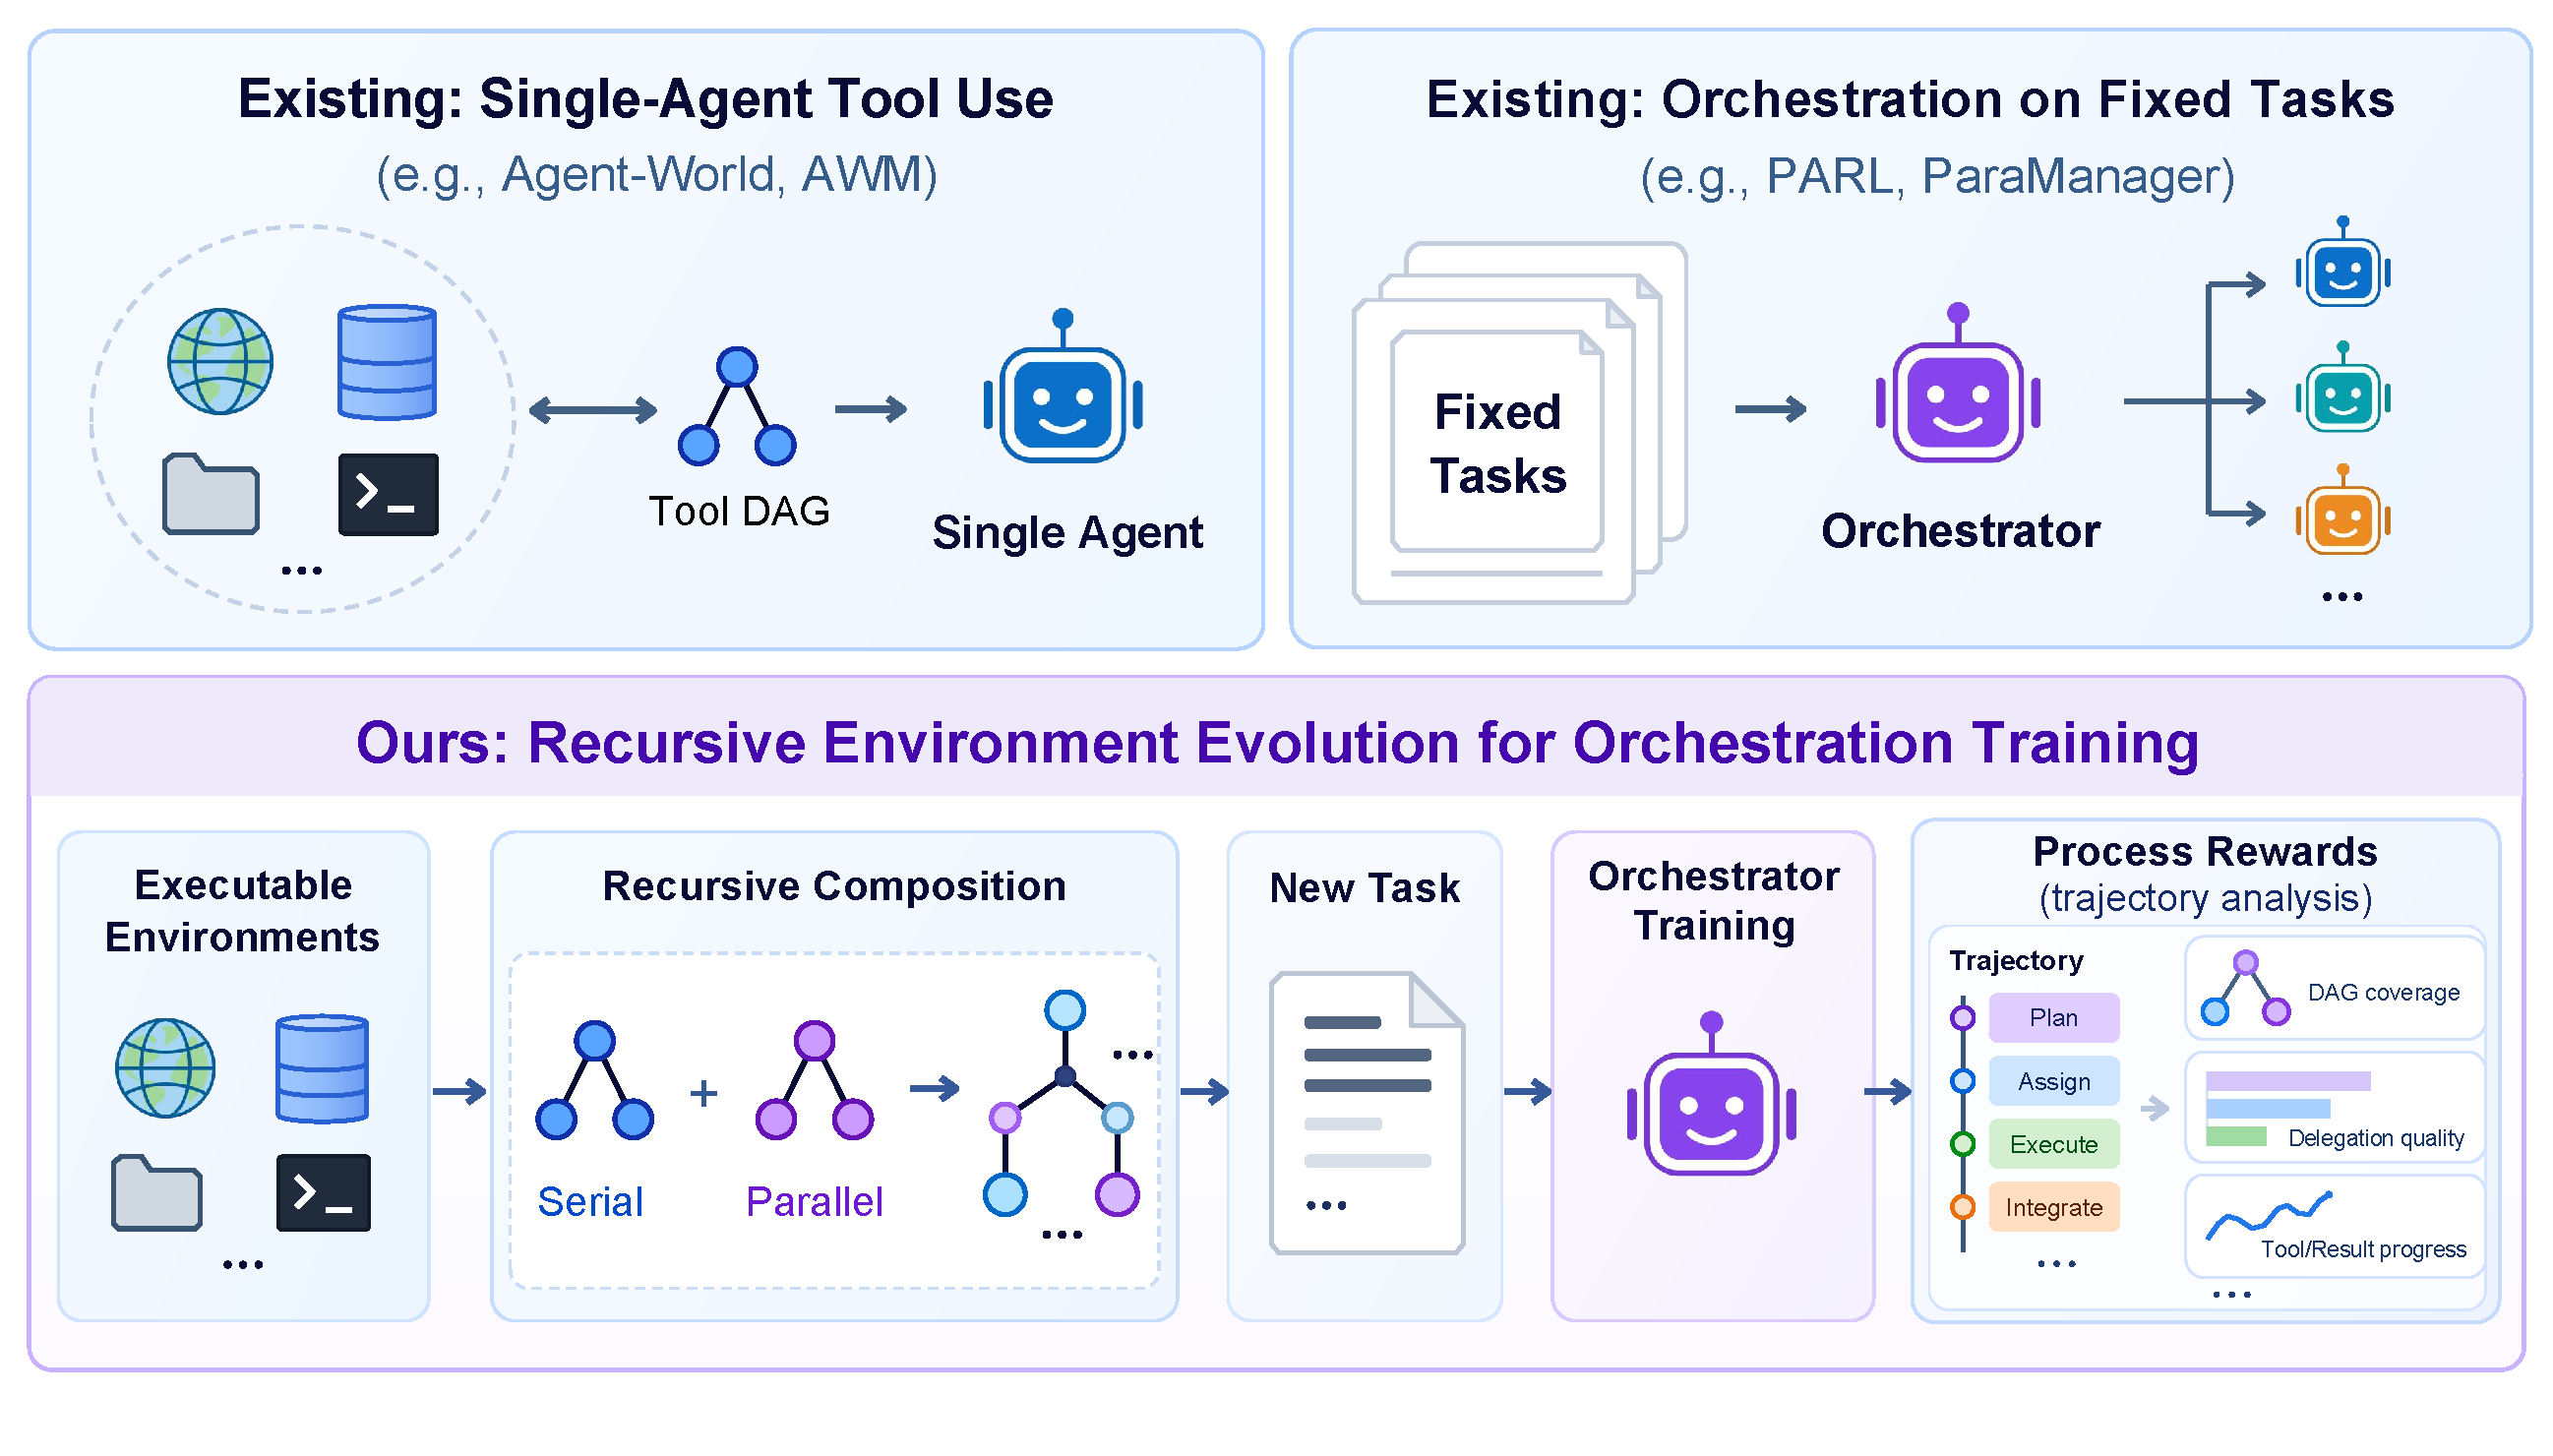
\includegraphics[width=0.75\linewidth]{figures/figure1.pdf}
  \caption{\textbf{Environment requirements for orchestration training.} Executable tools, state, and a verifier support tool-use learning (left). Orchestration tasks expose subgoals linked by serial dependencies or parallel branches (center), supporting delegation and result integration (right). The workflows illustrate training requirements.}
  \label{fig:environment-requirements}
\end{figure}

Training environments determine which decisions an agent can practice and what feedback it receives. Agent World Model~\citep{wang2026agentworldmodelinfinity}, Agent-World~\citep{dong2026agentworld}, and ToolVerse~\citep{zhou2026toolverse} construct executable tools and verifiable tasks for tool-use training. Building on this setting, MAW focuses on composing functional goals into coherent requests that require coordinating serial dependencies and parallel branches (Figure~\ref{fig:environment-requirements}). The construction must preserve executable interactions and evidence for checking both progress and completion.

We introduce \textbf{Multi-Agent World (MAW)}, a framework that combines recursive environment evolution with reinforcement learning for orchestration (Figure~\ref{fig:maw-overview}). MAW represents reference tool calls and their dependencies as directed acyclic graphs (DAGs), then composes task candidates through serial and parallel operations. Semantic reconstruction turns the candidate graphs into coherent user requests. Executing the reconstructed reference and applying quality gates check feasibility and agreement among the request, answer, and database state. The accepted tasks support training in which an orchestrator assigns roles and subtasks to frozen workers. We combine final outcome verification with process feedback on tool progress, answer coverage, and task organization, and optimize the orchestrator with Group Relative Policy Optimization (GRPO)~\citep{shao2024deepseekmath}.

\begin{figure}[t]
  \centering
  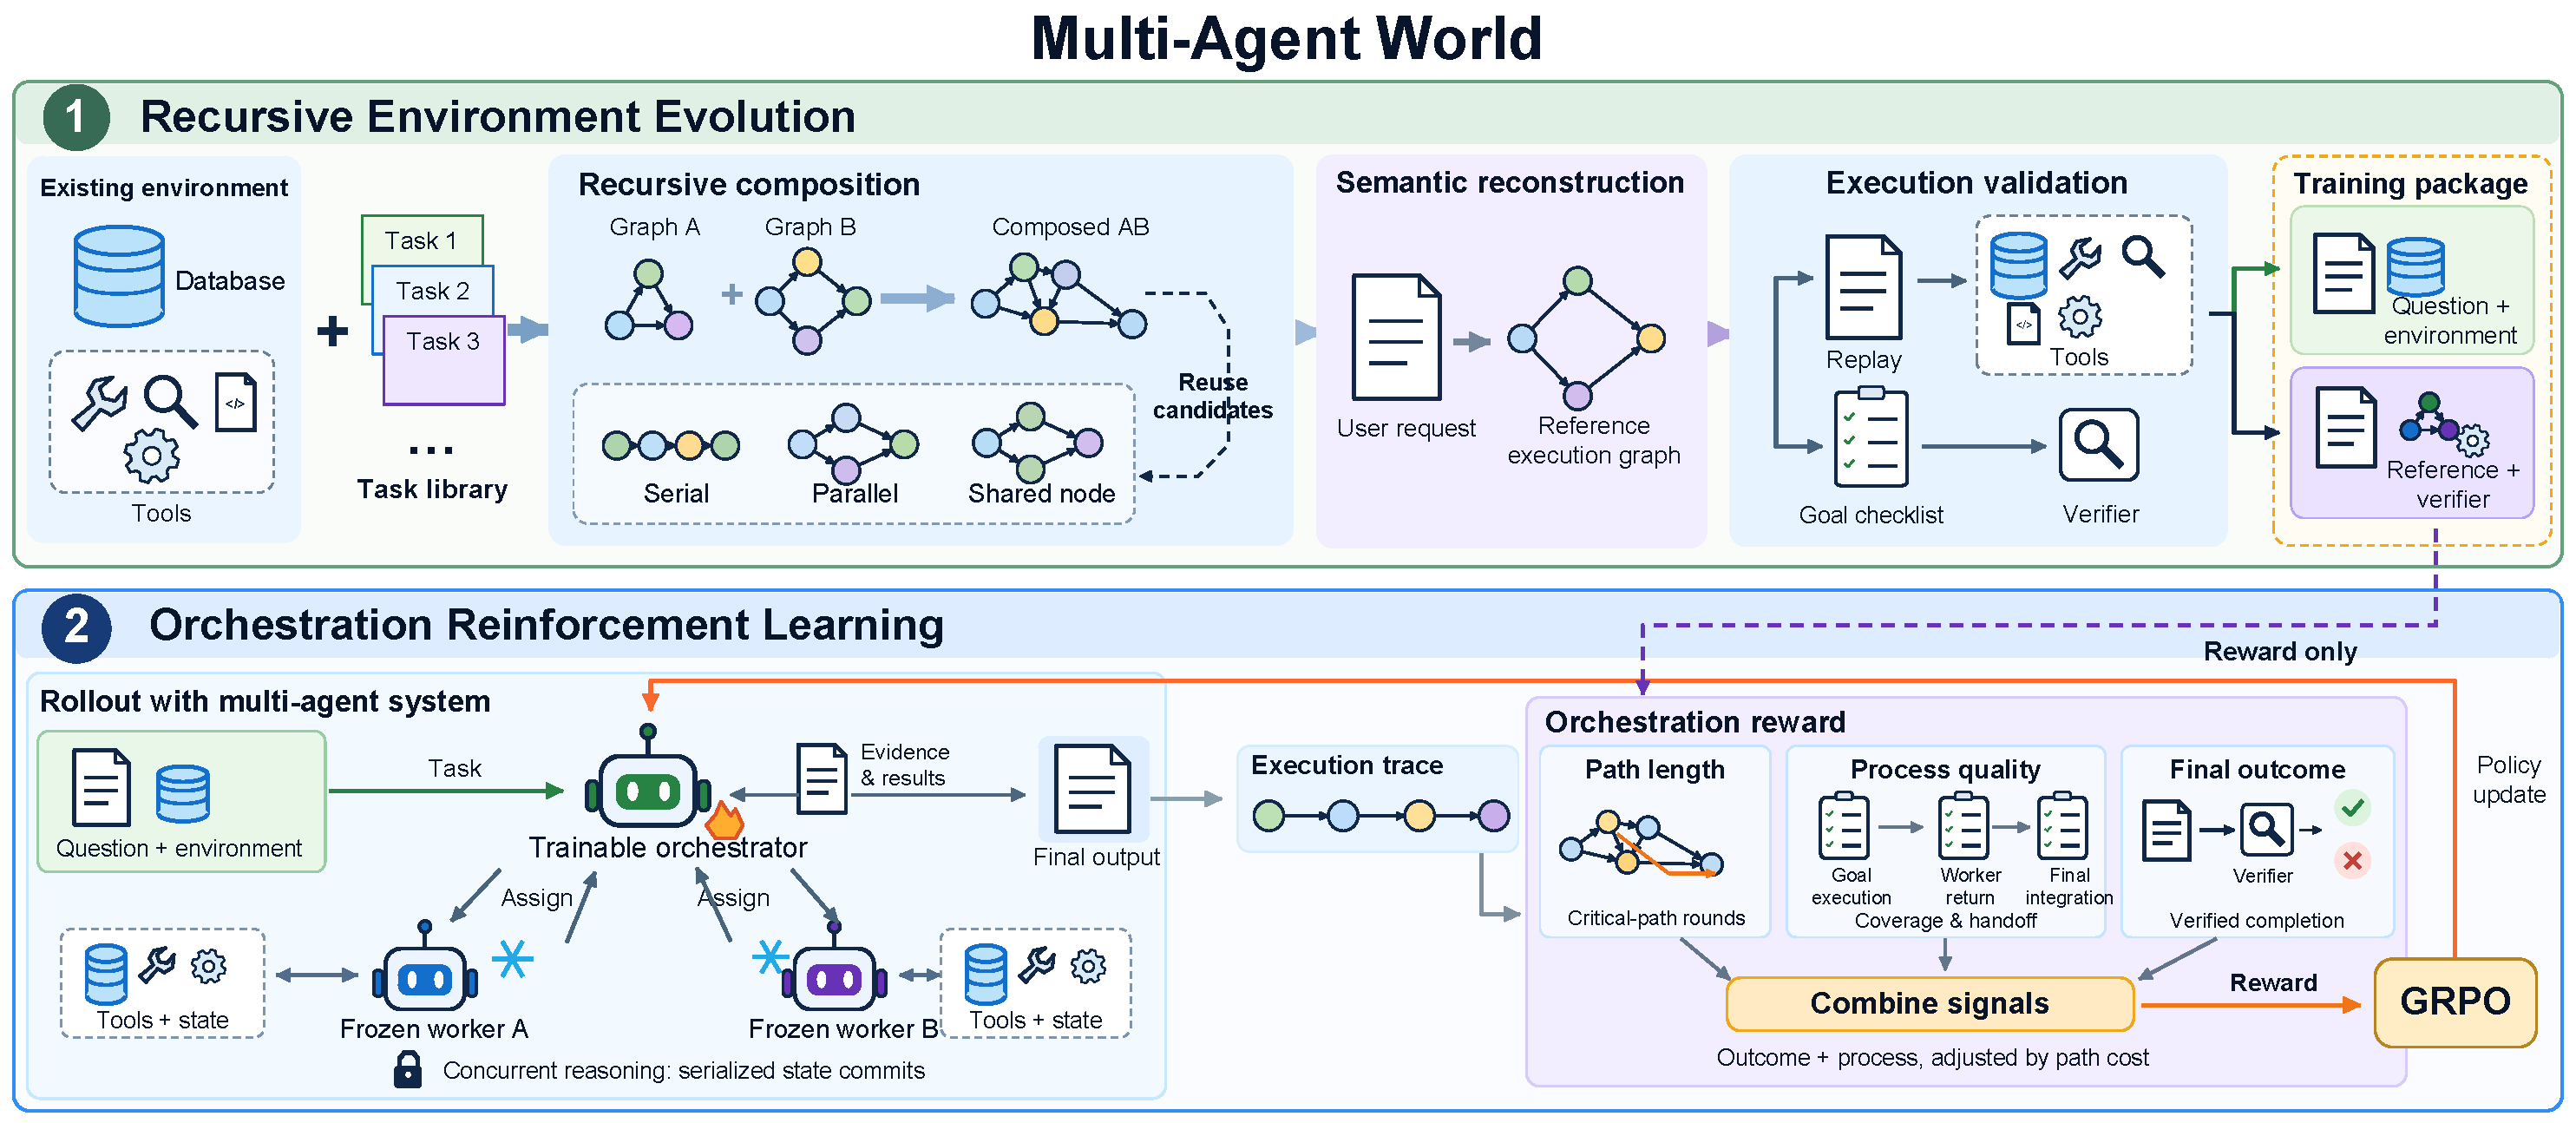
\includegraphics[width=\linewidth]{figures/figure2.pdf}
  \caption{\textbf{Overview of Multi-Agent World.} Task construction connects DAG composition, semantic reconstruction, execution, and quality gates. Accepted tasks provide resettable environments for interaction and hidden references for scoring. The orchestrator dynamically creates and reuses workers, combines their results, and receives a trajectory reward from outcome verification and process feedback. Only the orchestrator is updated.}
  \label{fig:maw-overview}
\end{figure}

Our evaluation examines task construction, transfer to external benchmarks, and the contribution of process feedback. The audited synthesis snapshot contains 2,581 accepted tasks in 539 environments; its comparison with the seed set is reported in Section~\ref{sec:composition}. Controlled training comparisons are designed to separate data-source effects from reward effects. \drafttodo{Report verified benchmark results and ablations; the synthesis counts alone do not establish training gains.}

Our contributions are as follows:
\begin{itemize}
  \item \textbf{Task construction for orchestration training.} We develop serial and parallel DAG composition, semantic reconstruction, and execution-based quality control to construct verifiable tasks within existing environments.
  \item \textbf{Orchestration RL with execution-grounded process feedback.} We combine final answer and database-state verification with feedback on tool progress, answer coverage, and delegated work to train the orchestrator.
  \item \textbf{Evaluation of task construction and orchestration learning.} We compare the seed and synthesized task sets and specify controlled data and reward comparisons. \drafttodo{Replace the planned learning comparisons with their measured findings.}
\end{itemize}

\section{Preliminaries: Executable Environments for Orchestration}
\label{sec:preliminary}

Following the executable-environment setting of AWM and Agent-World~\citep{wang2026agentworldmodelinfinity,dong2026agentworld}, we write an environment as $E=(\mathcal S,\mathcal U,T,s_0,\mathcal X,V)$. Here, $\mathcal S$ is the database-backed state space, $\mathcal U$ is the tool interface, and $T(s_t,a_t)=(s_{t+1},o_{t+1})$ executes a tool call and returns an observation. Each rollout starts from $s_0$ on a task $x\in\mathcal X$, with $V_x$ checking its answer and relevant state.

MAW extends this setting to $E^{\mathrm{orch}}=(\mathcal S,\mathcal U,T,s_0,\mathcal X^{\mathrm{orch}},\mathcal H,\widetilde V)$, where $\mathcal H$ lets an orchestrator delegate subgoals to workers acting on the shared environment. The expanded task set $\mathcal X^{\mathrm{orch}}$ composes multi-step subtasks. For a joint trajectory $\tau$ with answer $y_\tau$ and final state $s_\tau$, verification becomes $\widetilde V_x(\tau)=(V_x^{\mathrm{ans}}(y_\tau),V_x^{\mathrm{state}}(s_0,s_\tau),P_x(\tau))$. Beyond answer correctness, $V_x^{\mathrm{state}}$ checks the environment's full database state for required updates and unexpected changes, since worker reports can omit side effects. The trajectory-level feedback $P_x$ evaluates subgoal progress, evidence handoff, and integration, providing graded supervision for orchestration.


\section{Recursive Environment Evolution}
\label{sec:evolution}

MAW expands the task distribution within existing executable environments. It composes reference task graphs, reconstructs coherent user requests, and accepts tasks only after strict execution and quality checks. 

\subsection{Recursive Task Composition}
\label{sec:composition}

\paragraph{Seed tasks and task graphs.}
Our seed construction follows the executable-tool and graph-guided synthesis approach illustrated by ToolVerse~\citep{zhou2026toolverse}: real MCP tool schemas guide the construction of mock databases and executable tool functions, tool-graph sampling proposes call sequences, and execution provides evidence for reverse task synthesis. Each seed supplies a functional goal and a reference task DAG $H=(N,A)$, whose nodes represent tool-call instances and whose edges represent data or state dependencies. Composition operates on tasks from a compatible environment.

Let $\mathcal C_0$ be the seed pool. At round $r$, $\operatorname{Compose}_z$ combines compatible candidates in $\mathcal C_r$, where $z\in\{\mathrm{serial},\mathrm{parallel}\}$. Retained candidates can be used in later rounds, allowing a composite task to acquire further goals and dependencies. The provenance record preserves its parent tasks for tracing the construction.

\paragraph{Serial composition.}
Serial composition connects goals through an output or state effect required by a downstream operation. A first subtask may identify the records that a second subtask must inspect, or create an object that it subsequently modifies. The proposed edge must correspond to a usable dependency in the reconstructed execution. An arbitrary ordering between independent calls does not provide this dependency.

\paragraph{Parallel composition.}
Parallel composition combines goals that can progress independently before their results are integrated into a joint report, comparison, or decision. Compatible reads may be shared during reconstruction, but shared work is not a third composition operator. Calls are merged only when their arguments and state assumptions support the same use; matching tool names alone is insufficient.

Applying these two operators recursively produces candidates with mixed serial and parallel structure. The candidate DAG guides reconstruction; its size does not determine the number of calls required by the final task. Figure~\ref{fig:task-statistics} therefore compares seed references with reconstructed, accepted references. The audited snapshot uses two-parent candidates; its statistics do not measure gains from multiple recursive rounds (Appendix~\ref{app:synthesis}).

\begin{figure}[t]
  \centering
  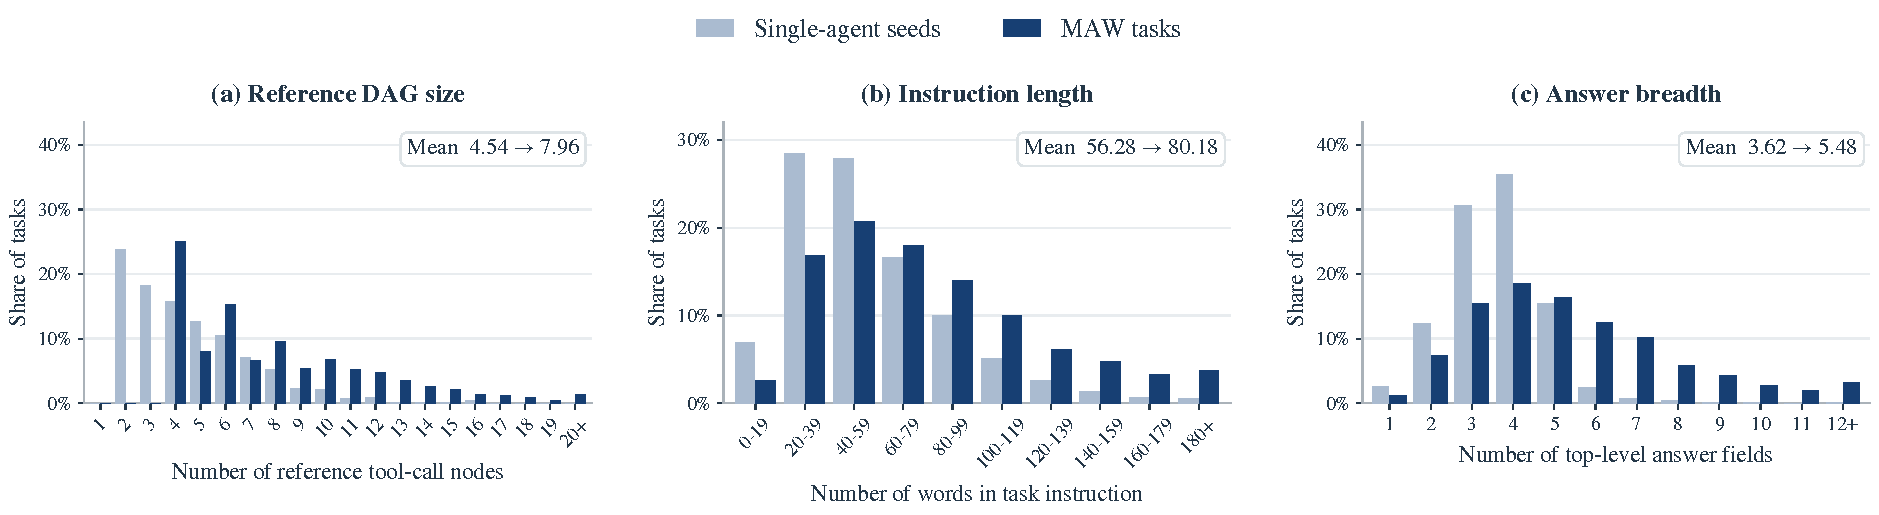
\includegraphics[width=\linewidth]{figures/task_statistics.pdf}
  \caption{\textbf{Seed and accepted-task statistics.}
Distributions of reference tool-call counts, instruction lengths (in words), and top-level answer-field counts for 10,860 seeds and 2,581 accepted MAW tasks.
Bars show the fraction of tasks within each cohort; inset labels report means (seeds $\rightarrow$ MAW).
For accepted tasks, reference tool-call counts are measured from the original reference DAGs before plan reconstruction.
Each cohort is normalized separately, and the final bin includes the full tail.
Answer-field counts exclude three seeds with non-dictionary answers.
These statistics describe the audited snapshot and do not measure solver difficulty or training benefit.}
  \label{fig:task-statistics}
\end{figure}

\subsection{Semantic Reconstruction}
\label{sec:reconstruction}

Graph composition specifies how reference operations may be connected, but does not yet provide a coherent user request. Parent tasks can refer to different entities, time ranges, or reporting requirements. Semantic reconstruction uses the candidate DAG, parent goals, and executable tool context to formulate a single request, instantiate tool arguments, and construct a reference plan. It may align entities, remove redundant calls, or add a lookup needed to support the combined goal. The request states the desired outcome without exposing the reference plan or prescribing worker allocation.

The reconstructed plan is executed to derive the reference answer and required database effects. Where an explicit task DAG is available, its tool nodes, dependency edges, and answer node are checked against that plan and its observed execution. Reconstruction thus connects the proposed graph structure to an executable problem; all final structural statistics must refer to the reconstructed artifact.

\begin{figure}[t]
  \centering
  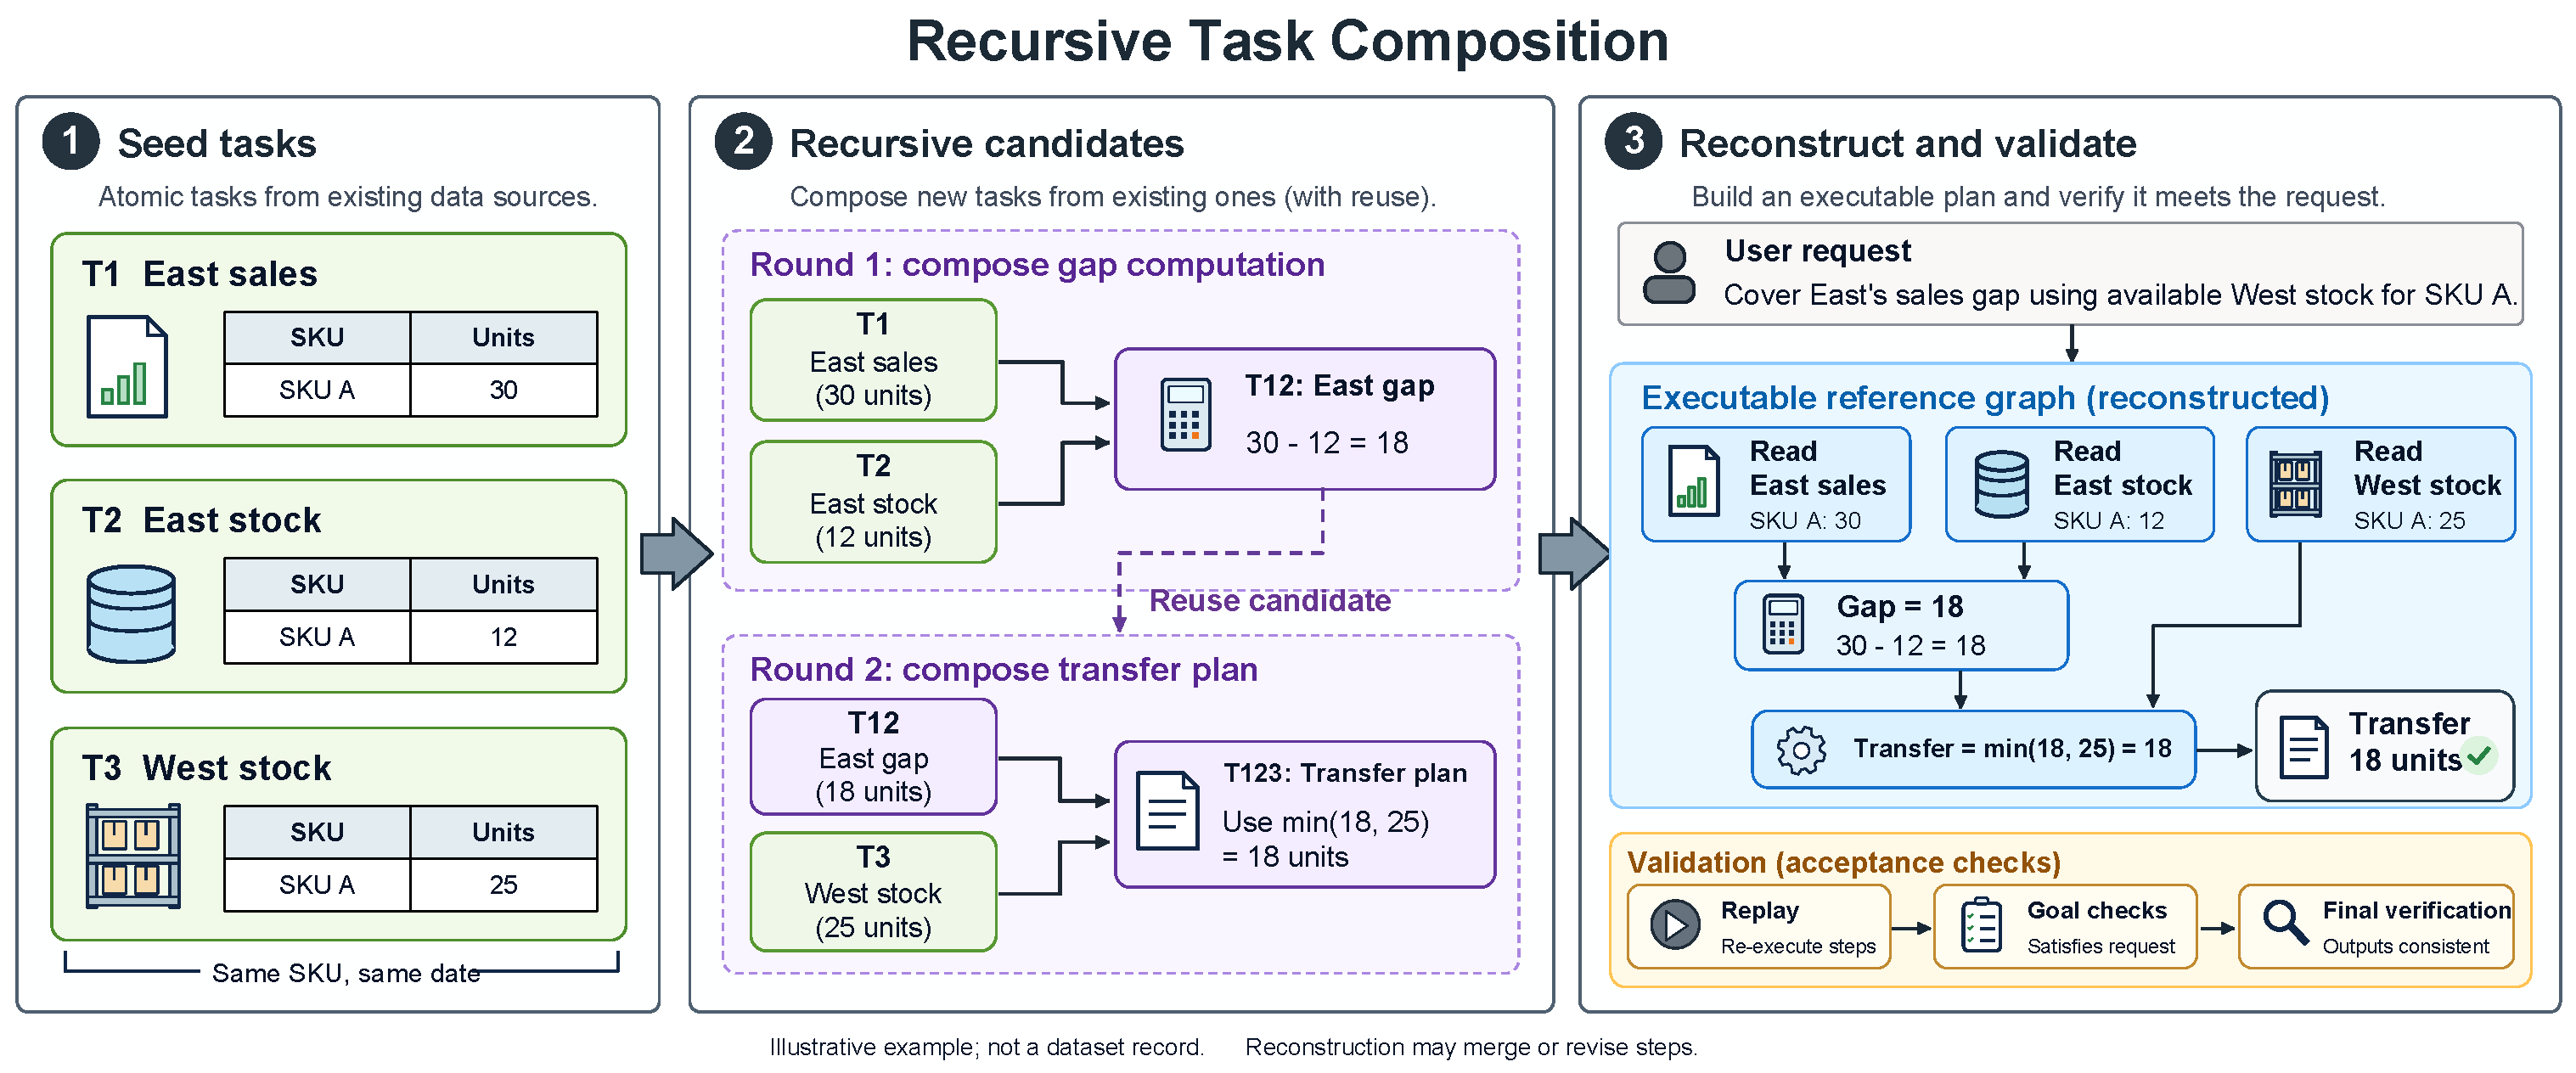
\includegraphics[width=\linewidth]{figure3.pdf}
  \caption{\textbf{DAG composition and semantic reconstruction.} Parent goals and reference operations provide the input. Serial or parallel composition proposes a candidate graph; reconstruction aligns its context into a coherent request and may revise the reference calls. Execution checks the resulting reference. The example illustrates the mechanism.}
  \label{fig:composition-example}
\end{figure}

\subsection{Execution and Quality Gates}
\label{sec:validation}

Repeated composition can accumulate redundant calls or combine incompatible requirements. MAW uses two levels of validation to keep these defects out of the accepted training set. \emph{Execution validation} first runs the reconstructed reference in an isolated, reset environment. It checks tool and argument validity, computes the answer from actual observations, and records final database changes. The generated solution is then replayed from the same initial conditions; its answer and final state must pass the checker.

\emph{Quality gates} assess whether this executable reference solves a coherent problem. They check fulfillment of the request, answer completeness, preservation of parent goals, workflow coherence, state consistency, and whether repeated operations serve a justified purpose. The audited pipeline requires two separate semantic reviews, each based on the request and execution evidence without seeing the other review's verdict. Both must pass every required check. A failed, uncertain, or missing review prevents acceptance. This screening adds semantic checks to successful execution, while retaining the possibility of shared errors by the review model.

An accepted task packages the request with its resettable environment, answer/state checker, and hidden reference evidence. These artifacts support both rollouts and process scoring. Construction provenance and exact acceptance records are retained separately from policy-visible inputs. Appendix~\ref{app:synthesis} documents the snapshot and its validation coverage.

% \begin{algorithm}[t]
% \caption{Recursive task construction and acceptance}
% \label{alg:synthesis}
% \begin{algorithmic}[1]
% \REQUIRE Seed pool $\mathcal C_0$, executable environments, composition budget $B$
% \STATE $\mathcal C\gets\mathcal C_0$; $\mathcal D\gets\varnothing$
% \WHILE{composition budget remains}
%   \STATE Select compatible parents and $z\in\{\mathrm{serial},\mathrm{parallel}\}$
%   \STATE Compose a candidate DAG and record its parent tasks
%   \STATE Reconstruct a coherent request and executable reference
%   \STATE Execute and replay the reference; verify the answer and final state
%   \IF{execution checks and all required quality gates pass}
%     \STATE Add the task package to $\mathcal D$; retain the candidate for later composition
%   \ENDIF
% \ENDWHILE
% \RETURN $\mathcal D$ and construction/acceptance records
% \end{algorithmic}
% \end{algorithm}

% Algorithm~\ref{alg:synthesis} describes the recursive construction path. The separately audited snapshot freezes its two-parent candidates before reconstruction; the distinction is recorded in Appendix~\ref{app:synthesis}.

\section{Orchestration RL with Execution-Grounded Process Rewards}
\label{sec:learning}

Terminal verification determines whether a task is complete, but provides little differentiation among incomplete rollouts. MAW supplements this outcome signal with evidence of tool progress, answer coverage, and the organization of delegated work. These components form one trajectory reward for the orchestrator.

\subsection{Multi-Agent Interaction Harness}

Given a user request and the available tool descriptions, the orchestrator $\pi_\theta$ dynamically assigns each worker a role and an allowed tool subset through \texttt{create\_subagent}. A registered worker can be reused for later subtasks of the same role. The orchestrator uses \texttt{assign\_task} for an individual assignment and \texttt{assign\_tasks} for concurrent assignments whose results are returned together. It integrates the returned evidence and terminates the episode with \texttt{submit\_answer}.

The orchestrator accesses task tools through workers. Each worker follows the frozen policy $\pi_\phi$, executes its assigned task with the authorized tools, and returns its findings. The runtime records tool events, assignment ownership, and returned results for scoring. Worker generations and tool observations form part of the orchestrator's context but are masked from its policy loss. Appendix~\ref{app:runtime} gives the interface and information boundaries.

\subsection{Answer and Database-State Verification}
\label{sec:outcome}

For a trajectory $\tau$ with final answer $y_\tau$ and state $s_\tau$, the binary outcome reward requires valid completion, an accepted answer, and the required database state:
\begin{equation}
 O(\tau)=\mathbf 1[\mathrm{valid\ completion}]
 \mathbf 1[V_x^{\mathrm{ans}}(y_\tau)=1]
 \mathbf 1[V_x^{\mathrm{state}}(s_0,s_\tau)=1].
 \label{eq:outcome}
\end{equation}
The answer checker evaluates the requested output fields and values. The state checker verifies required final mutations and rejects unexpected final changes. For a read-only task, the database must remain unchanged.

State verification is needed when a request contains several database operations: a plausible answer does not establish that a record was created, an update was applied, or unrelated data were preserved. Checking the actual final state prevents these omitted operations from receiving outcome credit solely because the response text is correct. Outcome verification constrains the requested result; it does not require the policy to reproduce the reference call sequence.

\subsection{Execution-Grounded Process Feedback}
\label{sec:process}

Process feedback examines progress at three levels: which required tool operations have been completed, how much of the requested answer is present, and whether delegated work produces evidence that reaches the final response. The score is grounded in recorded execution, worker returns, and the hidden reference.

\paragraph{Tool progress.}
The tool score $M$ measures coverage of validated reference milestones. A milestone receives credit when the actual execution contains a successful tool event with matching arguments and observations under the supported normalization rules. Dependency checks require the relevant predecessor evidence to be available. Repeated calls do not add coverage for an already matched milestone.

\paragraph{Answer coverage.}
The answer score $Q$ gives partial credit for correctly reported results. For dictionary answers, each top-level key--value pair is one row. Scalar and structured values use exact matching; lists use one-to-one element matching, with fractional credit for a partial match. If $m$ is the equivalent number of matched rows and $n_g,n_c$ are the reference and candidate row counts, we use
\begin{equation}
 Q=\frac{m}{n_g}\left(0.8+0.2\frac{m}{n_c}\right).
 \label{eq:answer-coverage}
\end{equation}
Empty or invalid submissions receive zero. This recall-oriented score distinguishes partial answers, while the binary outcome still requires full answer and state acceptance.

\paragraph{Organization and integration.}
Delivery $D$ measures whether workers return the evidence required by their assigned goals. The collaboration score $S$ combines useful goal allocation with evidence handoff and final-answer integration. It penalizes duplicate or irrelevant assignments and limits credit when required results are missing from the final answer. Independent-goal allocation is scored only on references that pass the required dependency and execution-order checks. Stateful or unsupported tasks use conservative progress scoring. These checks use actual events and returned content rather than self-reported completion.

For the supported branch, the process reward is
\begin{equation}
 P(\tau)=F\bigl(0.25M+0.25Q+0.20D+0.30S\bigr),
 \label{eq:process}
\end{equation}
where $F\in[0,1]$ measures compliance with explicit ordering constraints in the request. Each component lies in $[0,1]$. Here $S$ includes the integration adjustment to allocation credit; Appendix~\ref{app:process} specifies this notation and the fallback cases. Reference matching can under-credit correct alternative solutions, so process credit supplements outcome verification.

\subsection{Trajectory Reward and Policy Optimization}
\label{sec:objective}

The final reward prioritizes verified task completion:
\begin{equation}
 R(\tau)=O(\tau)+\lambda_pP(\tau),\qquad\lambda_p=0.3.
 \label{eq:reward}
\end{equation}
A successful rollout receives at least $1$, whereas an unsuccessful rollout receives at most $0.3$. Partial progress can therefore distinguish failed rollouts without outweighing successful completion. Execution cost is reported as an evaluation metric and does not enter this training reward.

For each task, we sample $G=8$ independently reset trajectories under the behavior policy and compute group-relative advantages:
\begin{equation}
 A_i=\frac{R_i-\overline R}{\operatorname{std}(R_1,\ldots,R_G)+\epsilon}.
 \label{eq:advantage}
\end{equation}
GRPO~\citep{shao2024deepseekmath} applies a clipped policy objective to the orchestrator's generated tokens, using the same trajectory advantage for all those tokens. Worker parameters remain fixed. The process score enriches the trajectory return; it does not assign separate advantages to workers or individual turns. Appendix~\ref{app:training} gives the optimization objective and configuration.

\section{Experiments}
\label{sec:experiments}

The evaluation separates three questions: whether the complete system transfers to external tasks, whether the synthesized data support useful orchestration, and whether the reward improves learning beyond outcome-only optimization. Tables~\ref{tab:main-results}--\ref{tab:training-ablation} define these comparisons. \textbf{Draft status:} the requested synthesis snapshot has been audited, but the final benchmark and training-ablation results are not yet available; their result cells remain placeholders, and the following text specifies the evaluation protocol rather than completed empirical findings.

\subsection{Experimental Setup}

\paragraph{Data and models.}
The documented development configuration uses Qwen3-8B~\citep{yang2025qwen3}, with both orchestrator and worker initialized from the same single-agent checkpoint. The audited synthesis snapshot contains 2,581 accepted tasks across 539 environments. An earlier training import contains 2,577 tasks; the four-record difference requires an ID-level import audit and is not treated as a held-out split. The final experiments require a frozen training/validation/test manifest, including task provenance and environment overlap checks. Checkpoint selection uses validation performance only. Workers remain frozen across MA comparisons. Appendix~\ref{app:training} records known settings and identifies the remaining configuration fields.

\paragraph{Benchmarks.}
The working seven-benchmark roster comprises WideSearch~\citep{wong2025widesearch}, DeepPlanning~\citep{zhang2026deepplanning}, MCP Atlas~\citep{bandi2026mcpatlas}, Toolathlon~\citep{li2025toolathlon}, BFCL multi-turn~\citep{patil2025bfcl}, $\tau^2$-Bench~\citep{barres2025tau2bench}, and Terminal-Bench 2.0~\citep{merrill2026terminalbench}. The first four follow the project's existing evaluation integrations; BFCL and $\tau^2$-Bench measure complementary tool-use capabilities, while Terminal-Bench extends the evaluation to terminal tasks. Exact versions, splits, simulators, and metric keys are specified in Appendix~\ref{app:benchmarks} as a manifest to be finalized. Toolathlon-GYM is the execution adapter, not a separate benchmark. Function-calling accuracy and task success are kept in separate columns, and no average combines them. The protocol excludes test tasks and benchmark-derived references from synthesis, reward annotation, and model selection.

\paragraph{Baselines.}
\emph{Base} is the original tool-capable backbone without additional project training. \emph{Single-agent} is the project's trained single-agent checkpoint executed without workers. \emph{Multi-agent} uses that same checkpoint as an untrained-for-orchestration controller with frozen workers and the MAW runtime. \emph{AWM}~\citep{wang2026agentworldmodelinfinity} and \emph{EnvScaler}~\citep{song2026envscaler} train the same backbone on their respective released environment/task resources under a common outcome-based recipe and evaluate with the same single-agent harness. These controlled adaptations test training-resource utility, rather than reproducing every optimization detail of the original systems. \emph{MAW} adds recursive task construction and orchestration RL. Main-table comparisons are system comparisons; only the controlled ablations isolate individual components.

\paragraph{Budgets and reporting.}
Every benchmark uses a shared total token cap, timeout, tool-access policy, and decoding configuration across methods, with an additional common worker-concurrency cap for MA systems. Actual orchestrator and worker tokens are both counted. Task failures and policy timeouts stay in the denominator; infrastructure failures are logged separately and handled by a predeclared rerun policy. We report benchmark-native quality metrics and retain per-task logs for paired comparisons. Efficiency reporting includes logical critical-path rounds, total tokens, and wall-clock time over all episodes. Appendix~\ref{app:statistics} defines aggregation and uncertainty estimation.

% Snapshot: 2026-09-23T18:39:36.670856+08:00; provenance: analysis/eval_tables_20260923_1839/results_snapshot_20260923.md
\begin{table*}[t]
\caption{\textbf{Agentic tool-use benchmarks.} Native accuracy (\%). * marks a partial or provisional snapshot (23 September 2026); rates use scored cases and exclude ungraded errors. BFCL Overall uses all scored cases available so far. MAW ACEBench is English MultiTurn only. Missing settings remain pending. ToolVerse parentheses retain the supplied gains over the Qwen3-8B reference.}
\label{tab:agentic-tool-use}
\label{tab:main-results}
\centering
\scriptsize
\renewcommand{\arraystretch}{1.12}
\setlength{\tabcolsep}{3pt}
\resizebox{\textwidth}{!}{%
\begin{tabular}{@{}lrrrrrrrrrrrr@{}}
\toprule
\multicolumn{1}{l}{Model} & \multicolumn{5}{c}{BFCL Multi-Turn} & \multicolumn{4}{c}{$\tau^2$-Bench} & \multicolumn{3}{c}{ACEBench-Agent} \\
\cmidrule(lr){2-6} \cmidrule(lr){7-10} \cmidrule(l){11-13}
& Base & MissFunc & MissParam & LongContext & Overall & Airline & Retail & Telecom & Overall & MultiStep & MultiTurn & Overall \\
\midrule
\multicolumn{13}{l}{\textnormal{Frontier Models}} \\
DeepSeek-V3.2 & 41.50 & 39.50 & 33.50 & 35.00 & 37.39 & 63.80 & 81.10 & 96.20 & 80.37 & 92.50 & 68.75 & 80.62 \\
GPT-4.1 & 47.50 & 32.50 & 32.50 & 43.00 & 38.88 & 56.00 & 74.00 & 34.00 & 54.67 & 95.00 & 70.83 & 82.92 \\
Kimi-K2-Instruct & 62.00 & 41.00 & 44.50 & 55.00 & 50.63 & 56.50 & 70.60 & 65.80 & 64.30 & 85.00 & 73.33 & 79.17 \\
\midrule
\multicolumn{13}{l}{\textnormal{Open-Source Foundation Models}} \\
Qwen3-14B & 53.06* & \pending & \pending & 49.09* & 51.63* & \pending & \pending & \pending & \pending & \pending & \pending & \pending \\
Qwen3-8B  & 32.00 & 33.50 & 22.00 & 28.00 & 28.88 & 22.00 & 43.20 & 18.40 & 27.87 & 53.44 & 39.58 & 46.51 \\
\midrule
\multicolumn{13}{l}{\textnormal{Open-Source Environment Scaling Methods}} \\
AWM & \pending & \pending & \pending & \pending & \pending & \pending & \pending & \pending & \pending & \pending & \pending & \pending \\
EnvScaler & 65.50 & \pending & \pending & 68.22* & 66.45* & \pending & \pending & \pending & \pending & \pending & \pending & \pending \\
ToolVerse (w/ TARA) & 51.50 & 38.50 & 28.50 & 31.50 & 37.50\,(+8.62) & 26.00 & 50.00 & 21.10 & 32.37\,(+4.50) & 60.00 & 63.33 & 61.66\,(+15.15) \\
\midrule
MAW (ours) & 53.26* & \pending & \pending & \pending & 53.26* & \pending & 48.44* & \pending & \pending & \pending & 41.70* & \pending \\
\bottomrule
\end{tabular}%
}
\end{table*}

\begin{table*}[t]
\caption{\textbf{Long-horizon benchmarks.} DeepPlanning is split into Shopping and Travel; cells show case accuracy followed by the partial-credit score in parentheses (all \%). Shopping averages over cases; Travel averages the two language settings. WideSearch reports item F1. MCPMark reports native pass rate on the filesystem setting. * marks partial or provisional results: MAW Travel has 225/240 scored reports (15 missing reports contribute zero to the full-domain metric), WideSearch has 15/200 failed cases scored as zero, and MCPMark has 39/40 graded cases.}
\label{tab:long-horizon}
\centering
\footnotesize
\renewcommand{\arraystretch}{1.15}
\setlength{\tabcolsep}{4pt}
\begin{tabular*}{\textwidth}{@{\extracolsep{\fill}}lcccc@{}}
\toprule
Model & \multicolumn{2}{c}{DeepPlanning: Acc. (Partial)} & WideSearch & MCPMark FS \\
\cmidrule(lr){2-3}
& Shopping & Travel & item F1 & Pass rate \\
\midrule
\multicolumn{5}{l}{\textnormal{Frontier Models}} \\
DeepSeek-V3.2 & \pending & \pending & \pending & \pending \\
GPT-4.1 & \pending & \pending & \pending & \pending \\
Kimi-K2-Instruct & \pending & \pending & \pending & \pending \\
\midrule
\multicolumn{5}{l}{\textnormal{Open-Source Environment Scaling Methods}} \\
AWM & \pending & \pending & \pending & \pending \\
EnvScaler & \pending & \pending & \pending & \pending \\
ToolVerse & \pending & \pending & \pending & \pending \\
\midrule
\multicolumn{5}{l}{\textnormal{Open-Source Orchestrator Methods}} \\
Tool Orchestrator & \pending & \pending & \pending & \pending \\
ParaManager & \pending & \pending & \pending & \pending \\
MAW (ours) & 4.17 (47.03) & 0.00 (18.75)* & 18.77* & 12.82* \\
\bottomrule
\end{tabular*}
\end{table*}


\subsection{Main Results: Task Quality and Execution Efficiency}

Table~\ref{tab:main-results} compares transfer across the seven task families. Base versus Single-agent measures the effect of the existing single-agent training stage. Single-agent versus Multi-agent evaluates adding the orchestration runtime without an orchestration update. Multi-agent versus MAW holds worker quality and interface fixed and tests the additional MAW training stage. AWM and EnvScaler provide executable-synthesis baselines for the complete system. These contrasts must be read alongside training cost and actual inference consumption, rather than attributed entirely to a single reward component.

The final analysis will report absolute differences within each benchmark, uncertainty intervals, and any regressions. A quality improvement accompanied by more computation supports a different conclusion from an improvement at lower cost. Appendix~\ref{app:extended-results} provides the corresponding per-benchmark efficiency table. \drafttodo{Insert the measured benchmark differences and cost tradeoffs; state which comparisons are supported by paired uncertainty estimates.}

\subsection{Orchestration Benefit and Training-Data Utility}
\label{sec:orchestration-experiments}

Table~\ref{tab:orchestration} separates the execution architecture from the training source. A versus B and C versus D compare SA and MA training on the same source, using outcome-only rewards. A versus C and B versus D compare AWM and MAW data within an architecture at matched training set size and budget. The AWM--MAW source comparison includes differences in task and environment distribution; it is not a pure test of recursion. E versus D measures outcome-only orchestration training from the unchanged initialization, while E versus F evaluates the full training objective. F versus G holds trained weights fixed and measures the effect of permitting concurrent assignments at inference. It does not identify a training effect.

% Snapshot: 2026-09-23T18:39:36.670856+08:00; provenance: analysis/eval_tables_20260923_1839/results_snapshot_20260923.md
\begin{table*}[t]
\caption{\textbf{Orchestration capability ablation on DeepPlanning.} Quality is case accuracy (partial-credit score), in \%. *: partial/provisional snapshot, 23 September 2026. Claude + Claude Shopping covers 50/120 scored cases; MA-8B + SA-8B Travel covers 225/240 reports. $C$ is reconstructed logical model rounds; time is mean inference seconds per recorded episode. Tokens are recorded-usage lower bounds. Cost coverage, harness versions, and budgets vary across these development runs.}
\label{tab:orchestration}
\centering
\footnotesize
\renewcommand{\arraystretch}{1.15}
\setlength{\tabcolsep}{4pt}
\begin{tabular*}{\textwidth}{@{\extracolsep{\fill}}llcccc@{}}
\toprule
Setting & Configuration & Acc. (Partial) $\uparrow$ & $C\downarrow$ & Time (s) $\downarrow$ & Tokens (k) $\downarrow$ \\
\midrule
Shopping & SA-8B (single-agent) & 2.50 (26.89) & $14.5$* & $26.4$* & $\geq 119.0$* \\
 & Claude (single-agent) & 33.33 (74.44) & $18.6$* & $159.4$* & $\geq 566.3$* \\
 & MA-8B + SA-8B & 4.17 (47.03) & $18.6$* & $84.6$* & \pending \\
 & Claude + SA-8B & 9.17 (56.77) & $58.3$* & $303.0$* & $\geq 782.1$* \\
 & MA-8B + Claude & \pending & \pending & \pending & \pending \\
 & Claude + Claude & 42.00 (79.50)* & $62.2$* & $556.5$* & $\geq 1142.8$* \\
\midrule
Travel & SA-8B (single-agent) & \pending & $10.3$* & $36.0$* & $\geq 128.8$* \\
 & Claude (single-agent) & \pending & $8.7$* & $96.0$* & $\geq 361.9$* \\
 & MA-8B + SA-8B & 0.00 (18.75)* & $15.1$* & $143.6$* & \pending \\
 & Claude + SA-8B & \pending & $106.1$* & $225.9$* & $\geq 652.8$* \\
 & MA-8B + Claude & \pending & $10.8$* & $227.4$* & $\geq 143.5$* \\
 & Claude + Claude & \pending & $35.0$* & $274.2$* & $\geq 403.5$* \\
\bottomrule
\end{tabular*}
\end{table*}


To isolate construction choices, a second data study holds the underlying environments, synthesis model, and outcome-only MA training recipe fixed. It compares original seeds, direct task synthesis, one-round composition, recursive serial-only composition, recursive parallel-only composition, and full recursion. We evaluate both valid-task yield at a fixed synthesis budget and downstream quality at an equal number of accepted training tasks. These tests distinguish producing more usable data from producing more useful data. Appendix~\ref{app:synthesis} defines acceptance denominators, lineage statistics, and the table for this study.

Structural analysis counts accepted functional goals, dependencies, shared work, and eligible independent goal pairs. Candidate node counts are not substituted for post-reconstruction structure. A held-out trace audit measures useful assignments, duplicated goal allocation, missing evidence, and final goal omissions. These diagnostics test the intended behavior; delegation count alone cannot establish orchestration quality. \drafttodo{Report the matched-data contrasts, construction ablations, and held-out behavior measurements without inferring a benefit from task complexity alone.}

\subsection{Training-Strategy Ablations}

Table~\ref{tab:training-ablation} compares outcome-only training with the full outcome-plus-process reward. Component ablations remove tool-progress credit, answer-coverage credit, or collaboration feedback while keeping the remaining coefficients fixed. All arms share the task set, initialization, frozen workers, training budget, and evaluation instances. Execution cost remains an evaluation metric in every arm.

% Snapshot: 2026-09-23T18:39:36.670856+08:00; provenance: analysis/eval_tables_20260923_1839/results_snapshot_20260923.md
\begin{table*}[t]
\caption{\textbf{Framework ablation on DeepPlanning.} Shopping and Travel are separate settings; quality is case accuracy (partial-credit score), in \%. The data comparison replaces MAW synthetic data with AWM data; the reward comparison contrasts outcome-only $O$ with outcome-plus-process $O+P$. The full MAW $O+P$ rows reuse the r11\_482 + SA1550 reference run identified in the experiment plan. * marks provisional values; unmeasured training variants remain pending.}
\label{tab:training-ablation}
\centering\footnotesize
\renewcommand{\arraystretch}{1.15}
\setlength{\tabcolsep}{3pt}
\resizebox{\textwidth}{!}{%
\begin{tabular}{@{}llllcccc@{}}
\toprule
Setting & Layer & Training data & Architecture / reward & Acc. (Partial) $\uparrow$ & $C\downarrow$ & Time (s) $\downarrow$ & Tokens (k) $\downarrow$ \\
\midrule
Shopping & Data & AWM & MA+SA / $O+P$ & \pending & \pending & \pending & \pending \\
 & Data & MAW synthetic (ours) & MA+SA / $O+P$ & 4.17 (47.03)* & $18.6$* & $84.6$* & \pending \\
 & Reward & MAW synthetic (ours) & MA+SA / $O$ & \pending & \pending & \pending & \pending \\
 & Reward & MAW synthetic (ours) & MA+SA / $O+P$ (ours) & 4.17 (47.03)* & $18.6$* & $84.6$* & \pending \\
\midrule
Travel & Data & AWM & MA+SA / $O+P$ & \pending & \pending & \pending & \pending \\
 & Data & MAW synthetic (ours) & MA+SA / $O+P$ & 0.00 (18.75)* & $15.1$* & $143.6$* & \pending \\
 & Reward & MAW synthetic (ours) & MA+SA / $O$ & \pending & \pending & \pending & \pending \\
 & Reward & MAW synthetic (ours) & MA+SA / $O+P$ (ours) & 0.00 (18.75)* & $15.1$* & $143.6$* & \pending \\
\bottomrule
\end{tabular}%
}
\end{table*}


The component ablations set the corresponding contribution to zero without redistributing its weight. For unsupported scoring branches, the same conceptual component must be removed consistently; each intervention requires a separate implementation/configuration binding before execution. We report goal coverage and evidence delivery with their supported-task denominators, alongside success under the unchanged final verifier. A larger process score alone is not higher task success. \drafttodo{Complete the reward-branch bindings and report measured ablation results.}

\section{Related Work}
\label{sec:related-work}

\paragraph{Executable environments and task synthesis.}
AWM synthesizes code-backed environments with structured state and verification for agent RL~\citep{wang2026agentworldmodelinfinity}. EnvScaler separates environment skeleton construction from scenario and rule-based validator generation~\citep{song2026envscaler}. Agent-World combines environment/task discovery with a diagnostic training loop~\citep{dong2026agentworld}, while ToolVerse uses tool dependencies to construct long-horizon tasks and turn-aware training signals~\citep{zhou2026toolverse}. EnvHarness modifies existing environments through interface components~\citep{huang2026envharness}, and SPADE learns an environment-design role through self-play~\citep{liu2026spade}. These approaches already support forms of composition, long-horizon interaction, or adaptation. MAW instead focuses on recursively composing functional goals within existing backends and retaining execution evidence for orchestration training. Its offline candidate recursion is distinct from policy-conditioned environment generation or an online diagnostic loop.

\paragraph{Multi-agent orchestration and reinforcement learning.}
AutoGen and MetaGPT organize collaboration through agent conversations and role-based workflows~\citep{wu2023autogen,hong2023metagpt}. Learned coordination is also established: evolving orchestration trains a controller for agent collaboration~\citep{dang2025orchestration}, PARL trains parallel agent systems and considers critical steps~\citep{kimiteam2026kimik25}, and ParaManager learns unified agent/tool orchestration with parallel subtask decomposition~\citep{yuan2026paramanager}. MAW builds on learned orchestration and uses execution cost as an evaluation metric. Its focus is the connection between synthesized orchestration tasks and a reward that checks reference goals, worker evidence delivery, and final integration. Unlike turn-aware advantage estimation in ToolVerse, the process score enters a trajectory-level GRPO return. The controlled experiments distinguish this training objective from gains due to additional data or the execution architecture.

\section{Conclusion and Limitations}
\label{sec:conclusion}

We presented MAW, a framework that connects orchestration-task construction with feedback on how delegated work is executed. Recursive composition expands functional goals within existing environments; semantic reconstruction and execution-grounded validation turn these candidates into training tasks. An outcome-prioritized reward combines answer and database-state verification with tool progress, answer coverage, and collaboration feedback to train an orchestrator with frozen workers. The evaluation separates complete-system transfer, orchestration benefit, and training-strategy effects. \drafttodo{Add the principal measured findings after the six-benchmark evaluation and controlled ablations are complete.}

The method has several limits. Reference matching may under-credit correct alternative solutions, and independent-goal rewards apply only to a verified subset of tasks. Logical model rounds omit tool latency and generation length, so efficiency claims require separate wall-clock measurements. Offline recursive construction does not establish online co-evolution of environments and policies. The audited two-parent synthesis snapshot also does not establish the benefit of multiple recursive rounds. The current interface requires delegation, and evidence from one model scale with frozen workers cannot establish generality to unrestricted agent organizations or jointly trained teams. Generated environments and completion checks also require audits for semantic errors that successful replay may not expose.

\input{sections/9_statements}

\FloatBarrier
\bibliography{iclr2027_conference}
\bibliographystyle{iclr2027_conference}

\clearpage
\appendix
\section{Recursive Environment Evolution: Examples and Validation}
\label{app:synthesis}

The following cases illustrate how composition combines parent goals and how reconstruction turns the resulting reference graph into an executable task. Parent goals and observations are summarized for readability; generated requests and reference answers are reproduced in full.

\subsection{Composing goals with shared evidence}
\label{app:composition-case}

\begin{systembox}{Case 1 \quad Kong control-plane monitoring}
\textbf{Environment.} Control planes with routes and services, and groups of member control planes.

\casepart{Parent tasks and DAG transformation}
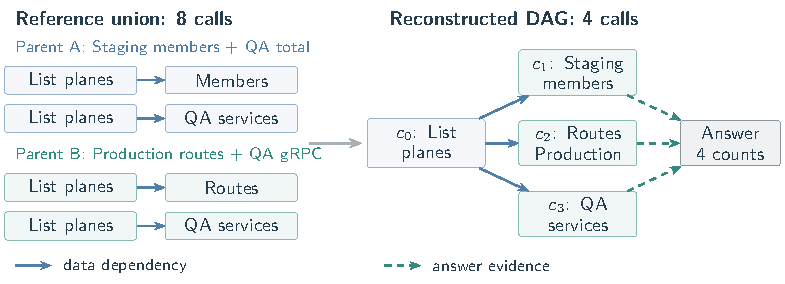
\includegraphics[width=\linewidth]{figures/synthesis_case_kong.pdf}

The two parent graphs form an eight-call reference union. Reconstruction merges the four discovery calls into one and the two QA-service queries into one, preserving all four requested counts.

\casepart{Generated request}
Find the control plane group named 'Staging' and count how many member control planes belong to that group. Then find the control plane named 'Production' with cluster type 'k8s' and count how many routes it has. Next, find the control plane named 'QA' with cluster type 'hybrid' in the 'ap-south' region and count both how many services are deployed to it and how many of those services use the 'grpc' protocol. Return the member count for the Staging group, the route count for Production, the total service count for QA, and the gRPC service count for QA.

\casepart{Reference execution \normalfont\small (all calls; condensed observations)}
\begingroup
\setlength{\tabcolsep}{3pt}\renewcommand{\arraystretch}{1.13}
\begin{tabularx}{\linewidth}{@{}l>{\raggedright\arraybackslash}p{.52\linewidth}Y@{}}
\toprule
 & Tool call & Observation \\
\midrule
$c_0$ & \texttt{list\_control\_planes()} & IDs: Staging group 2; Production/k8s 1; QA/hybrid/ap-south 5. \\
$c_1$ & \texttt{list\_control\_plane\_group\_memberships}\newline\texttt{(groupId=2)} & 2 member planes. \\
$c_2$ & \texttt{list\_routes(controlPlaneId=1)} & 30 routes. \\
$c_3$ & \texttt{list\_services(controlPlaneId=5)} & 10 services; 6 use gRPC. \\
\bottomrule
\end{tabularx}
\endgroup

\casepart{Reference answer and validation}
\noindent\begin{minipage}[t]{.64\linewidth}
\vspace{0pt}
\begin{lstlisting}[style=casejson]
{
  "staging_group_member_count": 2,
  "production_route_count": 30,
  "qa_total_service_count": 10,
  "qa_grpc_service_count": 6
}
\end{lstlisting}
\end{minipage}\hfill\begin{minipage}[t]{.32\linewidth}
\vspace{3pt}\raggedright
\textbf{State:} unchanged.\par\smallskip
\textbf{Passed:} execution, checker/replay, DAG checks, and both semantic reviews.
\end{minipage}
\end{systembox}
% Record: tc_kong_konnect_mcp_server:full:0002; parents S0003/S0015.
% Full parent requests, source node mappings and checker controls: evidence/cases/kong_case.json.
\begingroup\small
\refstepcounter{figure}\label{fig:composition-example}
\noindent\textbf{Figure \thefigure: Shared evidence across composed goals.} One discovery result supports three read branches; one service list answers both QA questions. The recorded execution is sequential.
\endgroup

\clearpage
\subsection{Pruning unused calls and restoring state order}
\label{app:reconstruction-case}

\begin{systembox}{Case 2 \quad Documentation refresh and search}
\textbf{Environment.} Documentation sources with crawl, indexing, and search operations.

\casepart{Parent tasks and DAG transformation}
Parent A refreshes the sources, counts enabled docs, and searches for ``hooks.'' Parent B refreshes the same sources, reports enabled docs and index size, and searches for ``error.''

\smallskip
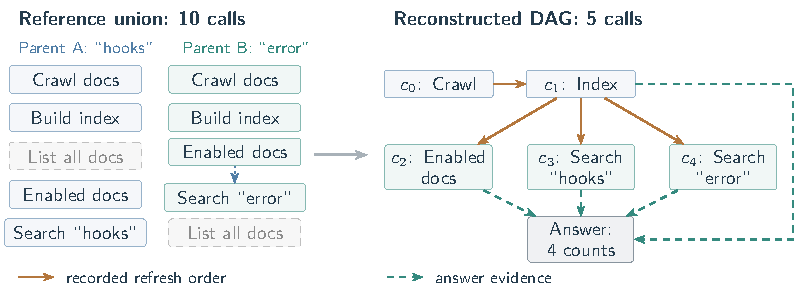
\includegraphics[width=\linewidth]{figures/synthesis_case_docs.pdf}

Reconstruction shares the crawl, index, and enabled-source calls, retains both searches, and removes the two \texttt{list\_all\_docs} calls (gray): their outputs add no requested result. The final DAG records refresh-before-query order. The dotted source edge is the only recorded candidate edge.

\casepart{Generated request}
Refresh the documentation search system by crawling all enabled documentation sources and rebuilding the search index. Then verify the system is working by checking how many documentation sources are currently enabled and indexed, and test the search functionality by querying for both 'hooks' and 'error'. Report the total number of enabled docs, total index entries created, and the number of search results found for each query term.

\casepart{Reference execution \normalfont\small (all calls; condensed observations)}
\begingroup
\setlength{\tabcolsep}{3pt}\renewcommand{\arraystretch}{1.13}
\begin{tabularx}{\linewidth}{@{}l>{\raggedright\arraybackslash}p{.52\linewidth}Y@{}}
\toprule
 & Tool call & Observation \\
\midrule
$c_0$ & \texttt{crawl\_docs()} & Enabled sources crawled. \\
$c_1$ & \texttt{build\_index()} & 10 docs indexed; 224 entries. \\
$c_2$ & \texttt{list\_enabled\_docs()} & 10 docs; all enabled, crawled, and indexed. \\
$c_3$ & \texttt{search\_docs(query='hooks')} & 2 matches. \\
$c_4$ & \texttt{search\_docs(query='error')} & 0 matches. \\
\bottomrule
\end{tabularx}
\endgroup

\casepart{Reference answer and validation}
\noindent\begin{minipage}[t]{.62\linewidth}
\vspace{0pt}
\begin{lstlisting}[style=casejson]
{
  "enabled_docs_count": 10,
  "index_entries_created": 224,
  "hooks_search_results": 2,
  "error_search_results": 0
}
\end{lstlisting}
\end{minipage}\hfill\begin{minipage}[t]{.34\linewidth}
\vspace{3pt}\raggedright
\textbf{State:} 10 docs updated; 24 pages and 224 index rows added.\par\smallskip
\textbf{Passed:} execution, checker/replay, DAG checks, and both semantic reviews.
\end{minipage}
\end{systembox}
% Record: tc_document_management_server:full:0006; parents S0009/S0010.
% Correspondences are inferred by matching operations, not a stored candidate-to-final node map.
% Recorded state order does not imply every reverse execution would fail.
\begingroup\small
\refstepcounter{figure}\label{fig:reconstruction-case}
\noindent\textbf{Figure \thefigure: Pruning and reconstruction.} Ten reference calls become five. Reconstruction also adds ordering edges, so the result is not a strict subgraph; the edges express the requested refresh order rather than a minimality guarantee.
\endgroup

\clearpage
\subsection{Execution and quality gates}
\label{app:synthesis-gates}

Table~\ref{tab:synthesis-gates} defines the acceptance checks. Failures trigger feedback and repair, with at most three generation attempts per candidate. Each attempt starts from a reset environment.

\begin{table}[H]
\centering\small
\caption{Quality gates and their acceptance conditions.}
\label{tab:synthesis-gates}
\renewcommand{\arraystretch}{1.17}
\begin{tabularx}{\linewidth}{@{}>{\raggedright\arraybackslash}p{.19\linewidth}Y@{}}
\toprule
Gate & Acceptance condition \\
\midrule
Plan validity & Allowed tools, valid arguments and unique call IDs; references resolve to earlier observations. \\
DAG consistency & One node per call plus an answer node; acyclic forward edges consistent with references and execution. State-order edges require evidence of a relevant state change. \\
Execution & Calls and answer computation succeed; tool contracts and database integrity hold. Contract-marked mutations change state. \\
Checker and replay & The checker accepts the reference and rejects corrupted answers and applicable state controls. Fresh-state replay reproduces the answer and required changes without unexpected mutations. \\
Semantic review & Both reviews pass all six criteria, cover both parents' outcomes, and leave no unresolved issue. \\
\bottomrule
\end{tabularx}
\end{table}

\begin{systembox}{Six semantic review criteria}
\setlength{\tabcolsep}{0pt}\renewcommand{\arraystretch}{1.2}
\begin{tabularx}{\linewidth}{@{}>{\bfseries\raggedright\arraybackslash}p{.32\linewidth}Y@{}}
Task fulfillment & Does execution accomplish the generated request? \\
Answer completeness & Does the answer include every requested result? \\
Parent preservation & Are both parents' functional outcomes retained? \\
Workflow coherence & Do the operations serve one coherent task? \\
State consistency & Do state claims agree with execution and the final database? \\
Justified repetition & Does each repeated call add information, observe changed state, or serve a distinct purpose? \\
\end{tabularx}
\smallskip
\textit{Condensed from the review protocol; every criterion requires supporting evidence.}
\end{systembox}

\noindent\textbf{Review setup and coverage.} The generator and both reviewers use Claude Sonnet 4.6. Review 2 sees no earlier verdict and runs only after Review 1 passes. All 2,581 accepted tasks pass both reviews; 2,037 also carry explicit question-DAG validation, while 544 follow the earlier policy.

\begin{figure}[H]
\centering
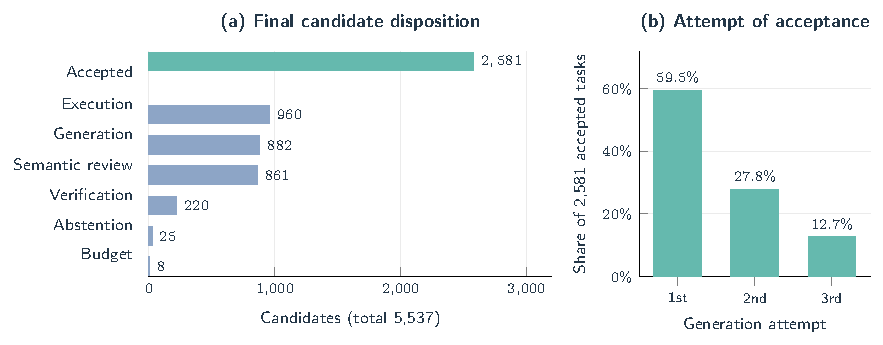
\includegraphics[width=.91\linewidth]{figures/synthesis_gate_outcomes.pdf}
\caption{\textbf{Candidate outcomes and repair.} Left: one final disposition per candidate, assigned to its last recorded stage, rather than a sequential filtering funnel. Right: successful attempt among 2,581 accepted tasks (46.61\%). Of these, 1,045 (40.49\%) pass after repair: 717 on attempt 2 and 328 on attempt 3.}
\label{fig:synthesis-gate-outcomes}
\end{figure}

\FloatBarrier

\clearpage
\subsection{Dataset profile and measurement definitions}
\label{app:synthesis-statistics}

The synthesis batch starts from 10,860 seeds across 598 environments and evaluates 5,537 two-parent reference unions. It yields 2,581 accepted tasks across 539 environments; 835 require state changes. The batch instantiates one composition round of the recursive procedure. Multi-round effects are left to the construction ablations below.

\begin{table}[H]
\centering\small
\caption{Mean reference structure before and after synthesis. The matched baseline is the mean of each accepted task's two parents, not their combined workload.}
\label{tab:synthesis-profile}
\setlength{\tabcolsep}{5pt}
\begin{tabularx}{\linewidth}{@{}Yrrrr@{}}
\toprule
Metric & All seeds & Matched parents & Accepted & Change \\
\midrule
Tool calls & 4.535 & 3.978 & 4.757 & +19.6\% \\
Distinct tools & 3.191 & 2.842 & 2.953 & +3.9\% \\
Answer fields & 3.623 & 3.483 & 5.478 & +57.3\% \\
\bottomrule
\end{tabularx}
\end{table}

\paragraph{Metric definitions.}
Tool calls count operations in the seed reference or reconstructed plan; distinct tools count unique tool names within that reference; answer fields count top-level dictionary keys. For task $i$, the matched baseline is $b_i=[m(p_{i1})+m(p_{i2})]/2$, and relative change is $100(\bar m/\bar b-1)$. A reused parent contributes once per descendant. The answer-field comparison excludes three non-dictionary seed answers and one affected parent pair, leaving 2,580 matched tasks. The corresponding mean over all 2,581 accepted tasks is 5.477, as shown in Figure~\ref{fig:task-statistics}.

\paragraph{Interpretation.}
The matched comparison measures how an accepted task differs from its own parents; the unconditional distributions describe the full seed and accepted populations. Both describe reference structure, rather than measured solver difficulty or training gains. The examples show recorded dependencies and request-consistent state order, without claiming minimal plans or measured parallel speedup. Reconstruction may merge, remove, or add operations and edges; strict-subgraph and counterfactual edge tests were not enabled in this batch.

\subsection{Construction ablations and structural measurements}

The construction experiment uses the same backend pool and generator for every row of Table~\ref{tab:construction-ablation}. Equal synthesis-budget runs measure accepted-task yield and cost per accepted task. Equal accepted-data runs measure downstream training utility with the same outcome-only MA learner. If a variant cannot supply the common task count, the experiment reduces all arms to their common feasible count or reports that arm separately; duplicating samples does not establish equal diversity.

\begin{table}[ht]
\centering\small
\caption{Construction ablations. Yield is accepted tasks per fixed generation budget; success is held-out task success after training on equal accepted-task counts. All values are pending.}
\label{tab:construction-ablation}
\begin{tabularx}{\linewidth}{Ycccc}
\toprule
Training-task source & Yield & Cost/task & Goals/task & Success (\%) \\
\midrule
Original seed tasks & \pending & \pending & \pending & \pending \\
Direct synthesis & \pending & \pending & \pending & \pending \\
One-round composition & \pending & \pending & \pending & \pending \\
Recursive serial-only & \pending & \pending & \pending & \pending \\
Recursive parallel-only & \pending & \pending & \pending & \pending \\
Full recursive composition & \pending & \pending & \pending & \pending \\
\bottomrule
\end{tabularx}
\end{table}

Planned structural measurements use the accepted reference: functional goals per task, required dependency relations, verified independent goal pairs, and shared evidence sources. We also report reference calls, but do not equate call count with task difficulty or rollout length. Lineage depth, ancestor count, reference-graph depth, and policy critical-path rounds are separate fields. Read-only independence must pass the order-validation procedure below before it is used for decomposition rewards.

\section{Runtime Interface and Information Boundary}
\label{app:runtime}

\subsection{Actions and execution semantics}

Table~\ref{tab:actions} describes the implemented orchestration actions. A worker is registered with a role description and a permitted tool subset. Single assignment is synchronous; batch assignment launches workers concurrently and returns after their results join. Worker reasoning can overlap, while tool state operations commit under a transaction lock. The observed implementation does not expose a general direct-tool action to the orchestrator, and its completion protocol requires at least one delegation. The manuscript therefore does not claim that it learns to choose between zero-worker execution and delegation.

\begin{table}[ht]
\centering\small
\caption{Orchestration action interface. Exact prompt and parser versions must accompany the final run manifest.}
\label{tab:actions}
\begin{tabularx}{\linewidth}{lY}
\toprule
Action & Required information and effect \\
\midrule
\texttt{create\_subagent} & Name, system prompt, and allowed tool names; registers a frozen-model worker. \\
\texttt{assign\_task} & Worker name and subtask prompt; executes one assignment and returns its result. \\
\texttt{assign\_tasks} & List of assignments; permits concurrent worker inference and joins their returns. \\
\texttt{submit\_answer} & Final answer in the required format; triggers completion and verification. \\
\bottomrule
\end{tabularx}
\end{table}

The paired MA baselines share tool schemas, role prompts, worker histories, truncation rules, and parser behavior. Serializing the trained policy replaces batch concurrency with ordered execution of its requested assignments, preserves output ordering, and logs any state-sensitive divergence. It is an inference intervention, not a new policy trained on serial traces. For stateful tasks, differences in returned observations can also change later decisions, so the intervention is not assumed to alter time alone.

\subsection{Visible and privileged information}

\begin{table}[ht]
\centering\small
\caption{Information boundary during an episode. Reward reports are not returned as observations.}
\label{tab:visibility}
\begin{tabularx}{\linewidth}{Yccc}
\toprule
Information & Orchestrator & Worker & Reward service \\
\midrule
User request & Yes & Assigned content & Yes \\
Allowed tool descriptions & Yes & Permitted subset & Yes \\
Actual tool/worker returns & Returned content & Own context & Logged content \\
Reference plan and expected answer & No & No & Yes \\
Verifier code and process contract & No & No & Yes \\
Milestone and reward-component scores & No & No & Yes \\
\bottomrule
\end{tabularx}
\end{table}

A leakage audit inspects the actual rendered requests and tool descriptions, not just source templates. The audit checks for reference answers, serialized reference graphs, verifier diagnostics, and accidental hidden-file access. Final train/test manifests also record normalized task text and source lineage. Tasks descending from the same seed family must be grouped before splitting; an environment-disjoint evaluation additionally groups all tasks from an environment. These checks are required for final experiments and are not represented as already completed by the existence of an import file.

\subsection{Event log and critical-path reconstruction}

Execution cost is a diagnostic, not a reward component in Eq.~\ref{eq:reward}. Let $w(v)=1$ for each orchestrator or worker generation event and zero for other events. With only causal parents retained, define
\begin{equation}
 d(v)=w(v)+\max_{u\in\operatorname{pa}_{\rm causal}(v)}d(u),\qquad C(\tau)=\max_{v\in G_\tau}d(v).
 \tag{B.1}\label{eq:critical-path}
\end{equation}
An empty maximum is zero. Edges representing only the serialized database commit order are excluded. The resulting logical model rounds omit tool latency and generation length; wall-clock time and total tokens are reported separately.


Every event needs an episode ID, event ID, actor, event kind, causal parent IDs, and any transaction-order parent. Model-generation events carry prompt/completion token counts and timing; tool events additionally record tool identity, normalized arguments, observation, status, and assignment ownership. Assignment start/end events connect worker execution to its returned result. Logs must preserve ordering and parent references so Eq.~\ref{eq:critical-path} can be recomputed independently of the reward hook.

For an illustrative fork--join execution, one orchestrator generation precedes two independent worker branches of lengths three and five, followed by one integration generation. Its critical path is $1+\max(3,5)+1=7$ model rounds; serializing those branches gives $1+3+5+1=10$. Both perform ten generations. These are arithmetic examples, not measured latency or accuracy results. Tool latency and generation length can make the corresponding wall-clock ratio very different from $10/7$.

\section{Process Reward: Matching Rules and Applicability}
\label{app:process}

\subsection{Tool and answer matching}

A reference milestone specifies a tool, canonical arguments, an observation digest, and supported aliases. Arguments are compared after filling declared defaults and applying explicitly listed environment-specific normalization rules. Observations are JSON-canonicalized when possible and hashed. Only successful matching events contribute coverage, with each reference milestone counted once. Information dependencies require available predecessor evidence; state dependencies also use execution order.

The recorded retrieval-window exception removes only \texttt{limit}, \texttt{max\_results}, \texttt{per\_page}, \texttt{page\_size}, and \texttt{show} from argument comparison. Both calls must be non-mutating; the actual observation must be nonempty JSON shorter than 12,000 characters and must retain the reference observation digest. This does not accept arbitrary broader queries or semantic paraphrases.

The answer score in Eq.~\ref{eq:answer-coverage} uses top-level key--value rows. A missing reference key receives zero; an extra candidate key increases the precision denominator. A scalar or structured value requires equality. List elements are matched one-to-one without reusing an element, and fractional list coverage contributes to the equivalent matched-row count. Empty or invalid submissions receive zero. Final binary acceptance remains governed by the task's answer/state checker.

\subsection{Allocation, delivery, and integration}

Independent-goal allocation is eligible only when the reference contains independent goal pairs, its milestones are non-mutating, and its order-proof record has three passing executions including a changed order. These tests establish eligibility for the supported scorer, not universal commutativity. Ambiguous reference occurrences do not receive guessed ownership.

Each credited goal must have one assignment owner. Repeated or empty instructions do not receive allocation credit. A legal exact attempt receives partial credit; a matched observation and a returned worker result provide full goal evidence. Pair scoring checks distinct ownership and causal independence of assignment boundaries, then discounts redundant or irrelevant allocation.

Answer-dataflow annotations connect supported goals to their source operands and final-answer components. Delivery checks whether the worker return contains the required raw evidence or a matching derived result. Integration checks the corresponding final-answer components and the whole answer. In Eq.~\ref{eq:process}, $S$ denotes allocation credit after delivery and integration adjustments. This notation absorbs the implementation's multiplicative integration adjustment; it does not add a reward component or remove the check for missing results. $D$ is mean supported-goal delivery.

\subsection{Fallbacks and implementation binding}

Stateful tasks, missing answer-dataflow support, or ambiguous references cannot be assigned the supported independent-goal formula unconditionally. The documented matching implementation uses conservative progress based on covered milestones, satisfied dependencies, productive assignments, returned evidence, and nonredundant tool events. Missing or mismatched mandatory reference artifacts are integrity errors, rather than policy failures.

The revised main text specifies the supported-branch weights and the cost-free reward from the author's annotated draft. Historical development formulas use different weights and must not be reused as the final fallback specification. \drafttodo{Bind the final reward module and configuration hashes, exact fallback coefficients, row-matching edge cases, and the number of tasks supported by each branch before reporting training results.}

\subsection{Outcome priority}

Under Eq.~\ref{eq:reward}, $O=1$ and $P\geq0$ imply $R_{\rm success}\geq1$. For a failed trajectory, $O=0$ and $P\leq1$ imply $R_{\rm failure}\leq\lambda_p=0.3$. Every verified success therefore outranks every failure under this scalar reward. This property assumes a correct outcome evaluator and bounded process scores; it does not guarantee policy convergence or an improvement in success rate.

\section{Optimization and Configuration}
\label{app:training}

Let $\mathcal T_i$ denote orchestrator-generated token positions in rollout $i$, and $\rho_{it}(\theta)$ the ratio of current to behavior-policy token probabilities under the recorded context. The clipped GRPO policy term can be written
\begin{equation}
 J(\theta)=\mathbb E\!\left[\frac1G\sum_{i=1}^{G}\frac1{|\mathcal T_i|}
 \sum_{t\in\mathcal T_i}\min\!\left(\rho_{it}A_i,
 \operatorname{clip}(\rho_{it},1-\epsilon_l,1+\epsilon_h)A_i\right)\right]
 -\beta\mathcal K(\theta).
 \tag{D.1}
\end{equation}
Here $\mathcal K$ denotes the configured KL regularizer. This expression states the policy-ratio objective; exact loss aggregation, KL estimator, and clipping settings must be bound to the final trainer configuration. Worker completions, tool returns, and other observations are excluded from $\mathcal T_i$. Their probability is not optimized through the orchestrator loss.

\begin{table}[ht]
\centering\small
\caption{Working training configuration. Earlier recorded settings are distinguished from the revised reward specification; the final run binding remains pending.}
\label{tab:configuration}
\begin{tabularx}{\linewidth}{YY}
\toprule
Setting & Recorded value \\
\midrule
Backbone & Qwen3-8B \\
Orchestrator initialization & Single-agent checkpoint (recorded rollout 1550) \\
Worker initialization/update & Same checkpoint / frozen \\
Imported training set & 2,577 tasks in the earlier import; final manifest pending \\
Optimization & GRPO; outcome + process reward \\
Task batch / rollouts per task & 16 / 8 \\
Training duration & 3 epochs planned; 483 updates planned \\
Process coefficient $\lambda_p$ & 0.3 \\
Cost in training reward & None \\
KL handling & Enabled in recorded process flags; coefficient to be frozen \\
Completion protocol & At least one delegation required \\
\bottomrule
\end{tabularx}
\end{table}

The revised reward weights follow the annotated manuscript; the earlier runtime snapshot supports the recorded interaction and masking behavior. These sources do not establish a completed run under the revised specification. Final experiments must bind model/checkpoint hashes, dataset/split hashes, reward code and configuration, completed updates, learning rate, KL estimator and coefficient, clipping bounds, loss aggregation, decoding, truncation, worker limits, timeouts, hardware, and compute. The 2,581 synthesized records and the earlier 2,577-record import require a separate ID-level reconciliation.

\section{Evaluation Manifest and Statistical Protocol}
\label{app:benchmarks}

\subsection{Benchmark identity and adapters}

Table~\ref{tab:benchmark-manifest} fixes the intended identities while exposing unresolved versions. The first four are supported by the project's evaluation inventory; Terminal-Bench 2.0 is selected from an existing experiment registration. BFCL and $\tau^2$-Bench extend coverage based on the earlier blueprint and related tool-use evaluations. This seven-column roster is a working choice, not an assertion that the author has frozen all seven protocols.

\begin{table}[ht]
\centering\footnotesize
\caption{Working benchmark manifest. Every final score requires a dataset revision, evaluator commit, subset manifest, and decoder configuration.}
\label{tab:benchmark-manifest}
\begin{tabularx}{\linewidth}{lYY}
\toprule
Benchmark & Metric and purpose & Version/adapter boundary \\
\midrule
WideSearch & Official item F1 as primary; whole-case accuracy separately & ByteDance-Seed/WideSearch; split and scorer commit pending. \\
DeepPlanning & Official \texttt{avg\_acc}; report task-family breakdown & Pin release, travel/shopping subsets, and aggregation rule. \\
MCP Atlas & Official claim-rubric pass rate; freeze coverage threshold & scaleapi/mcp-atlas; distinguish available-service subset from full benchmark. \\
Toolathlon & Official task success & Toolathlon-GYM adapter; pin task set, services, and evaluator. \\
BFCL multi-turn & Official multi-turn accuracy & Freeze BFCL version and category aggregation; do not mix v3/v4 scores. \\
$\tau^2$-Bench & Official task success at the declared trial protocol & Pin verified/original version, domains, user simulator, and repetitions. \\
Terminal-Bench 2.0 & Official task resolution & Pin 2.0 task revision and harness; do not substitute 2.1 or later scores. \\
\bottomrule
\end{tabularx}
\end{table}

The official project entry points include \href{https://github.com/ByteDance-Seed/WideSearch}{ByteDance-Seed/WideSearch}, \href{https://github.com/scaleapi/mcp-atlas}{scaleapi/mcp-atlas}, \href{https://github.com/eigent-ai/toolathlon_gym}{eigent-ai/toolathlon\_gym}, and \href{https://github.com/harbor-framework/terminal-bench-2}{harbor-framework/terminal-bench-2}. These identify resources, not immutable experimental versions. A main-table result must reference a frozen revision and explicit metric key. Source adapters may normalize tool-call syntax but must preserve task semantics, evaluator behavior, and information access.

\subsection{Paired estimates and costs}
\label{app:statistics}

The primary unit is the task. Within each benchmark, every method attempts the same instances under paired evaluation seeds and identical initial states where the benchmark permits deterministic reset. Multiple rollout seeds on a task are averaged before task-level aggregation. The proposed uncertainty protocol uses 10,000 paired bootstrap resamples of task IDs and reports percentile 95\% intervals for scores and method differences. For repeated training runs, training-seed variation is additionally reported and resampled hierarchically; evaluation-only intervals must not be described as training uncertainty. The final number of training and evaluation seeds remains to be declared.

For a benchmark with native domain weighting, the bootstrap preserves that aggregation rather than replacing it with a pooled task average. No average over heterogeneous benchmark metrics is used in the main table. Whole-task correctness is distinct from field-level accuracy, partial credit, or process reward. If significance tests are added, their hypotheses and multiplicity correction must be specified before interpreting many pairwise contrasts.

All-episode mean cost includes failed and timed-out attempts. We also report wall-clock median and 90th percentile, timeout frequency, total input/output tokens across every model, tool attempts, and peak active workers. Latency is measured from episode start to terminal answer or timeout under declared hardware and concurrency conditions. Environment reset and queueing costs are separately logged with an explicit inclusion policy. A both-success subset can diagnose speed differences but is secondary because conditioning on success can favor different populations.

Infrastructure exceptions, such as unavailable services or reset failures, are recorded separately from a valid trajectory that fails verification. A rerun policy must use the same inputs and count all replacement attempts in the audit. Persistent missing infrastructure is reported as coverage loss, not silently removed to improve a score. The final run ledger records attempted, completed, failed, timed-out, rerun, and unavailable episodes for each method.

\section{Extended Results and Behavior Audits}
\label{app:extended-results}

\begin{table}[ht]
\centering\small
\caption{Per-benchmark efficiency record for each method. Duplicate this block for Base, Single-agent, Multi-agent, AWM, EnvScaler, and MAW when results arrive. Values remain pending. Latency quantiles include the declared timeout handling.}
\label{tab:efficiency}
\begin{tabularx}{\linewidth}{Yccccc}
\toprule
Benchmark & Mean $C$ & Tokens (k) & Time p50 & Time p90 & Timeouts (\%) \\
\midrule
WideSearch & \pending & \pending & \pending & \pending & \pending \\
DeepPlanning & \pending & \pending & \pending & \pending & \pending \\
MCP Atlas & \pending & \pending & \pending & \pending & \pending \\
Toolathlon & \pending & \pending & \pending & \pending & \pending \\
BFCL multi-turn & \pending & \pending & \pending & \pending & \pending \\
$\tau^2$-Bench & \pending & \pending & \pending & \pending & \pending \\
Terminal-Bench 2.0 & \pending & \pending & \pending & \pending & \pending \\
\bottomrule
\end{tabularx}
\end{table}

Behavior audits use held-out MAW tasks with reference annotations. Coverage is the matched-goal fraction, delivery is the mean supported-goal delivery score, and duplicate allocation is excess assignment ownership per attempted goal. We report the fraction and count of tasks supporting each metric, including the subset eligible for independent-goal scoring. External benchmarks without such annotations receive only their official outcome scores and available runtime metrics; MAW process scores are not retroactively inferred from benchmark answers.

\begin{table}[ht]
\centering\small
\caption{Failure taxonomy for trace review. Labels may co-occur; their rates are not assumed to sum to 100\%.}
\label{tab:failures}
\begin{tabularx}{\linewidth}{lY}
\toprule
Failure class & Auditable criterion \\
\midrule
Goal omission & A required subgoal has no supporting execution evidence. \\
Duplicate work & Multiple assignments repeat a goal without new evidence or a required retry. \\
Dependency misuse & A consumer executes without the prerequisite information or state. \\
Handoff failure & A worker obtains relevant evidence but its return omits the required content. \\
Integration failure & Available branch results are omitted or incorrectly combined in the final answer. \\
Worker execution & Delegation is appropriate but local tool choice, arguments, or reasoning fail. \\
Budget exhaustion & The episode reaches the common token, step, or time limit before completion. \\
Environment/checker error & Replay, state behavior, or evaluation is inconsistent with the declared task. \\
\bottomrule
\end{tabularx}
\end{table}

Case reports should include the task ID, visible request, selected tool descriptions, assignment prompts, relevant tool observations, worker returns, final answer, verifier outcome, and actual execution graph. A successful and an unsuccessful case from each principal structure slice should be selected by a declared sampling rule rather than chosen solely for visual appeal. The reference may be shown post hoc for analysis, clearly separated from policy-visible content. Annotators review goal omission, dependency, handoff, and integration evidence separately and record disagreements. The case-study counts and agreement measurements remain pending.

\section{Availability, Ethics, and Author Declarations}
\label{app:declarations}

\paragraph{Data and code availability.}
The planned research package contains environment/reset manifests, task provenance, synthesis and acceptance code, reward-side annotations, prompts, baseline adapters, training configurations, and per-task evaluation logs. Public release URLs and licenses have not yet been finalized. Access to hidden evaluation references must remain separated from solver-facing assets. \drafttodo{Add the frozen repository commit, release location, license inventory, and access conditions.}

\paragraph{Ethics and limitations of use.}
Synthetic tool environments can contain unrealistic assumptions or faulty checks. They should be executed in isolated sandboxes and reviewed for copied private data, credential-like strings, and unauthorized external side effects before release. The task concerns agent training rather than a human-subject experiment; this statement does not replace an institutional determination where one is required. The same orchestration capability can coordinate harmful actions, so deployment requires tool-specific permissions and monitoring beyond the training reward.

\paragraph{Author contributions, conflicts, and funding.}
\drafttodo{Authors must supply their CRediT contributions, conflict-of-interest declaration, and funding acknowledgments. No declaration of absence is inferred.}

\paragraph{AI assistance.}
AI assistance was used to analyze supplied writing examples, draft and edit manuscript text, organize experimental tables, and check LaTeX consistency. Numerical experimental results were not generated to fill missing measurements. The authors remain responsible for reviewing technical claims, references, and experimental reporting. This working disclosure must be checked against the applicable submission policy before submission; no venue-policy compliance is asserted here.


\end{document}
